
\documentclass[12pt,a4paper,oneside]{book}
\usepackage{setspace}
\onehalfspacing
%\doublespacing
\usepackage[hmargin={3cm,3cm},vmargin={2.5cm,2.5cm}]{geometry}


\usepackage[english]{babel}
\usepackage[utf8]{inputenc}
\usepackage[T1]{fontenc}


\usepackage[final]{pdfpages} % include pdf files

\usepackage{amsthm}
\usepackage{amsmath}
\usepackage{amsfonts}
\usepackage{tabularx}
\usepackage[nottoc, notlot, notlof, numbib, numindex]{tocbibind}


\usepackage{url}
%\usepackage{geometry}
\usepackage{enumitem}
\usepackage{hyperref}
\usepackage{comment}
\usepackage{listings} 
\usepackage{caption} 
\usepackage{stmaryrd}
\usepackage{fancybox}
\usepackage{makeidx}

\usepackage{eurosym}
\usepackage{multirow}
\usepackage{adjustbox}
\usepackage{charter}
\usepackage{graphicx}
\usepackage{booktabs}
\usepackage{pdfpages}

%\usepackage[authoryear, square]{natbib}

\usepackage[backend=bibtex8,sorting=none]{biblatex} 
\addbibresource{../reference/bibliography.bib}


%\bibliographystyle{unsrt}

\newcommand{\bp}{\textit{Copark }}

\newcommand\T{\rule{0pt}{2.6ex}}       % Top strut
\newcommand\B{\rule[-1.2ex]{0pt}{0pt}} % Bottom strut


\begin{document}
%\maketitle


\begin{titlepage}
\noindent \begin{minipage}{0.83\textwidth}
\noindent \textbf{UNIVERSIDAD CARLOS III DE MADRID}\hfill{}\\
\textbf{Graduate School of Business}\hfill{}\\
\textbf{Master in Management}\hfill{}
\end{minipage}
\begin{minipage}{0.17\textwidth}

\includegraphics[keepaspectratio=true,width=\textwidth]{../images/logo_UC3M_universidad_Carlos_III_Madrid.jpg}
\end{minipage}
\begin{center}
\vfill{}\vfill{}\vfill{}
%\begin{center}
{\Huge Business Plan : Copark}
%\end{center}
{\Huge \par}
\begin{center}{\LARGE Simon \textsc{Picard}}\end{center}{\Huge \par}
%\vfill{}\vfill{}\vfill{}\vfill{}\vfill{}
\vfill{}

\includegraphics[keepaspectratio=true,width=\textwidth-2cm]{../images/Seal_of_the_University_of_Carlos_III.jpg}
\vfill{}
\begin{flushleft}{\large \textbf{Supervisor  :}}\\
{\large Prof. Kurt \textsc{Desender}}
\end{flushleft}{\large\par}
\vfill{}\vfill{}\enlargethispage{2cm}
\textbf{Academic year 2016~-~2017}
\end{center}
\end{titlepage}



\newpage
%\newgeometry{hmargin={3.5cm,1.5cm},vmargin={2.5cm,2.5cm}}
\thispagestyle{empty} 
\null

\frontmatter

\tableofcontents

\mainmatter

\chapter{Introduction}

\chapter{Industry Environment}
\label{iechap}

\section{Macro Environmental Analysis}

\subsection{Economic}
%According to the GDP per capita (PPP), the European Union is the second largest economy in the world. Its total GDP is \euro 16.5 trillion in 2016 , which represents 22.8\% of the global GDP\cite{imfgdp}. The 2008 financial crisis appears to be in the process of recovery, as the economy of 19 of its countries advanced by 0.6 percent over the first three months of the year, as compared to the previous quarter\cite{eurorecov}.\\

%Belgium's economy is mainly composed from the service sector, accounting for 74.9\% of its GDP. Belgium also profits from a heavy industrial sector, which is concentrated mainly in northern Flanders, around Brussels and in Liège and Charleroi. The industry sector represents 21.1\% of Belgium's GDP. Finally, the agriculture sector represents less than 1\% of its GDP.\\
With a GDP of \$508.6 billion (PPP, 2016), Belgium ranks itself at the 38th position of the richest country in the world. In 2016, the GDP growth was 1.4\% and the unemployment rate was 8.4\%.\\
With approximately two thirds of Belgium's GDP relying on exportation, the country relies heavily on world trade. This high proportion comes from its skilled, multicultural and central population\cite{ciafb}.\\

The economy of Brussels is mainly oriented around the service industry, with 88\% of all jobs being in the service sector. Brussels alone contributes to a fifth of Belgium's GDP. Brussels holds 550 000 jobs and it represents 17.7\% of the country employment. There are 2000 foreign company offices in the capital.\cite{bxinfo}.\\
Brussels is one of the richest cities of the world with a GDP per capita of 67,811 (PPP) in 2016, which ranks it at the 9th position within the raking of the city of the OECD\cite{oecdstat}, Brussels is thus the economic capital of the country. Brussels GDP is boosted by a number of commuters from nearby regions. There are 230 000 employees coming from Flanders and another 130 000 coming from Wallonia working in Brussels. On the other hand, only 16\% of Brussels inhabitants work outside of the city\cite{euresCom}.\\
Although having apparently a big wealth, Brussels is not the holder of all of it. Indeed, it appears that the proportion of the unemployed resident of Brussels was 20.4\% in December 2013.\cite{unemploybx}\citeauthor{unemploybx}

\subsection{Political and Legal}

%Belgium is a constitutional, popular monarchy and a federal parliamentary democracy. The country is divided in three regions, Wallonia, Flanders and Brussels, which all have regional government.\\
%The worldwide governance indicator gives us information about the political situation of Belgium. The indicators say that the Belgium is a country of low corruption, high government effectiveness, high regulatory quality, high rule of law and high voice and Accountability. Based on those indicators, Belgium lacks political stability and absence of violence/terrorism with a value in this indicator of 65 in 2015\cite{wbgi}. On the other hand, when compared with other western European countries such as Spain and France, Belgium is valued higher in this field.\\
%Part this political stability score can be explained by the language and regional division of the country and subsequently political opinions.\cite{bailo2016political}.\\

The Belgian employment laws are based on the consultation of employees and workers. The length of the work is limited to 8 hours per day and 40 hours per week. There is a minimal wage which is valued at \euro 1 501,82 (2015)\cite{eurostatmw}.\\
A potential new law known as "Peteers' Law" is being studied, which would make the maximal number of hours that one can work based annually instead of weekly. This would lead to a potential week of 45 hours.\cite{rtlp} This process shows a trend of work deregulation.\\

%As a member of the European Union, Belgium applies the "common customs tariff of the European Union" to goods imported from non-EU countries. Overall, Belgium is open to trade since the country itself relies heavily on it. The trade regulation is decreasing, as one can see from the rise of the European Union, CETA and TAFTA//TTIP. Although those regulations are not currently established, the trend is to facilitate the international trade, especially for Brussels, as the capital of Europe.\\

\subsection{Social}

Belgium as a total population of 11 250 000 (2016) inhabitants and it is growing at a rate of 0.82\% (2008). 66.3\% of the population is between 15 and 64 years old. Its largest city is Brussels, with a total population of 1 175 173\cite{ciafb}.\\

%A current social concern for Belgium is the integration of the second and third generations of immigrants. A part of this segment is not integrated to the country whether socioeconomically of culturally. This phenomenon concern principally groups of young Belgian citizens of Moroccan origin who feel excluded from the society, this is particularly happening in Brussels and Antwerp\cite{sgikc}.\\

As Belgium has 27,3\% of its population younger than 24 years old and its median age is 43.1 years, Belgium has a younger population emerging\cite{ciafb}. It is then relevant to investigate the trends for the millennial and surrounding generation to understand the rises of trends in Belgium. The millennial are highly connected through social media and mobile data. The generation Z is even more. As the first members of the generation Z will turn 21 years old in 2017, their influence will impact the market.\\
This super-connection leads to promotion over social media, platforms less shopping and digitalisation. Overall, what is needed is a fast process, with instant notification and picture based description of the product\cite{stbe}.



\subsection{Environmental}

Belgium has a high density of population which impacts its environment particularly in the major cities of the country. Overall, Belgium is oriented toward an environment-friendly approach, being ranked 41 out of 180 in the environment protection index\cite{epi} and Belgium has one the most efficient recycling process. In Flanders, 75 \% of the residential waste produced is reused, recycled or composted\cite{wastemana}.\\

In 2010, a study was conducted about the main means of transportation of Brussels inhabitants. The result was that, within Brussels, the car was used by 32\% of the population, and for movement to or from Brussels, the car was preferred in 63.6\% of the cases.\cite{mtpd}

\subsection{Technological}
As \bp is designed to be an on-demand application present on desktop computers but mainly mobile devices, several technological factors have an impact on the viability of the business.\\

Belgium has a well-developed internet infrastructure, and rank itself among the most connected country in the world. Belgium has 8.6 millions of internet users, which represent 82.0\% of the population.\cite{intuser} There is 3.6 million users of fixed broadband and 3.5 million subscribers of mobile broadband.\cite{intsub} The global coverage of houses is 99.96\% for a 1 Mpbs connection and 91.1\% for a 100 Mbps one.\cite{fixcov} Regarding the mobile coverage, the whole country is covered in 2G connection, almost all the country has access to the 3G network and most urban area have 4G connection.\cite{mobcov}\\

\bp would also rely on cloud technology for the host of the application and the needed computing power. There are lots of offers of hosting available and it does not rely on the location of the use of the application since Belgium has a fast strong internet coverage.\\

\bp would be part of the on-demand economy. This model is based on an online platform where independent sellers have an offer for another individual. Classic examples of this economy are \textit{Uber} and \textit{eBay}. Recent surveys and data show that this segment is growing and attracting more and more people, not just a young or wealthy population.\cite{odegrow}

\subsection{Conclusion}
This analysis allows us to see that Brussels is a suitable market for \bp.\\
From an economical point view, Brussels's population is wealthy enough to embrace the product. A big part of Brussels's economy comes from the service, which is an industry where there is often mandatory movement by car. Moreover, a lot of employees in Brussels come from outside the city.\\
From the political side, Belgium's government effectiveness is high and there is close to no corruption. Thus \bp would be safe from any sort of blackmail and its legalisation and regulation process would be on time. The business opportunity does not rely on a lot of employment thus the employment law is aligned with it.\\
The Belgium's population is not an old one and it is still growing. Thus the market size is not threatened. The younger generation is increasingly tech savvy which is correlated to the on-demand economy.\\
Environmentally speaking, Belgium is very conscious. As \bp will reduce non-utilised space, improve parking utilisation and prevent potentially new parking lot to emerge, its aim is linked to environmental issues.\\
Finally, Belgium is technologically able to receive the on-demand business. Indeed, the country is very well connected and hosting services are easily available within.

\section{Industry Description and Market Boundaries}
The parking industry is not a straightforward one, it can be free, private or publicly owned.\\
The obvious business offer is the parking offered through the big building designed only for that goal. Those are usually privately owned and are offering spots only in specific locations, usually key locations where there is a lot of demand.\\
Then there is the free parking in the street. When a driver wants to find a spot in the street, he would rely on luck and knowledge of the neighbourhood to find it. In rural or low-density area, finding a spot is not a problem as there is low demand. On the other hand, in dense area, the available spots are rather rare because in front of a house there would two spots for ten or more inhabitants, leading to an offer too small. Free parking is sometimes subject to time limits in crowded location, the driver could stay only two hours, for example. This process is used to facilitate car turnover.\\
In dense area, the parking is usually subject to charge for non-residents of the area. This was developed as a means to give more liberty to the inhabitant and incentive people to use another means of transportation than the car.\cite{nycar} In the same way as for the free parking, the maximum time of stay of non-free parking is sometime bounded to a few hours to increase the number of spots available.\cite{bxpay} \\
The other possibility is to buy a parking space in the street, this option is usually linked to a house. A similar process is to rent the space on a monthly basis. Those are approaches that are suitable for long-term use, typically when the user lives next to the parking spot and struggle to find free ones.

\subsection{Private Parking Short-Term Rent}
Parking problems arise in dense area, where there are a lot of inhabitants in the neighbourhood and too few available spots for all of them. A solution to this problem is to charge for parking spots for non-residents.\\
First of all, this solution is not perfect, the driver may still struggle to find a spot. Secondly, the parking would not be free for the user if he does not live in the area.\\

On the other hand, there are lots of empty private parking spaces. Indeed, houses often come with a garage and a parking space driveway but the owner might not have a car, leading to an empty space. More likely, the owner would not use the spot all the time. For example, if he works in an office, his parking spot would typically be free from 9 am to 5 pm.\\
The \autoref{mapentry} shows how many in street access are present in a selection of streets in the west of Brussels. As one can see, the amount of unused space is large.\\


\begin{figure}[h]
\centering
\caption{Access Private or Public Parking\cite{mapentrysrc}}
\label{mapentry}
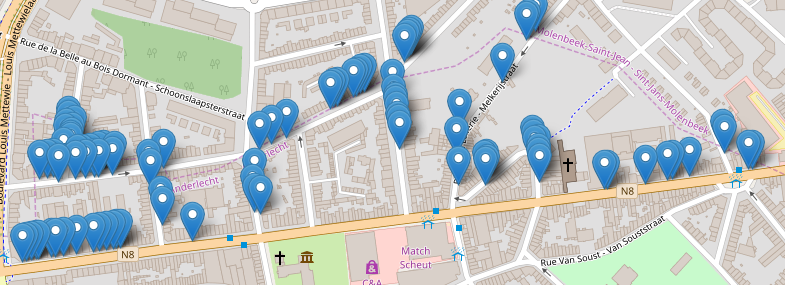
\includegraphics[keepaspectratio=true,width=\textwidth-2cm]{../images/casestudyander.png}
\end{figure}

The \autoref{ruexl} is a picture of a typical street in Brussels. As one can see, the street is full of cars and the only spots left are empty driveways.

\begin{figure}[h]
\centering
\caption{Avenue Général Médecin Derache, a street in Brussels at 5pm, April 2017}
\label{ruexl}
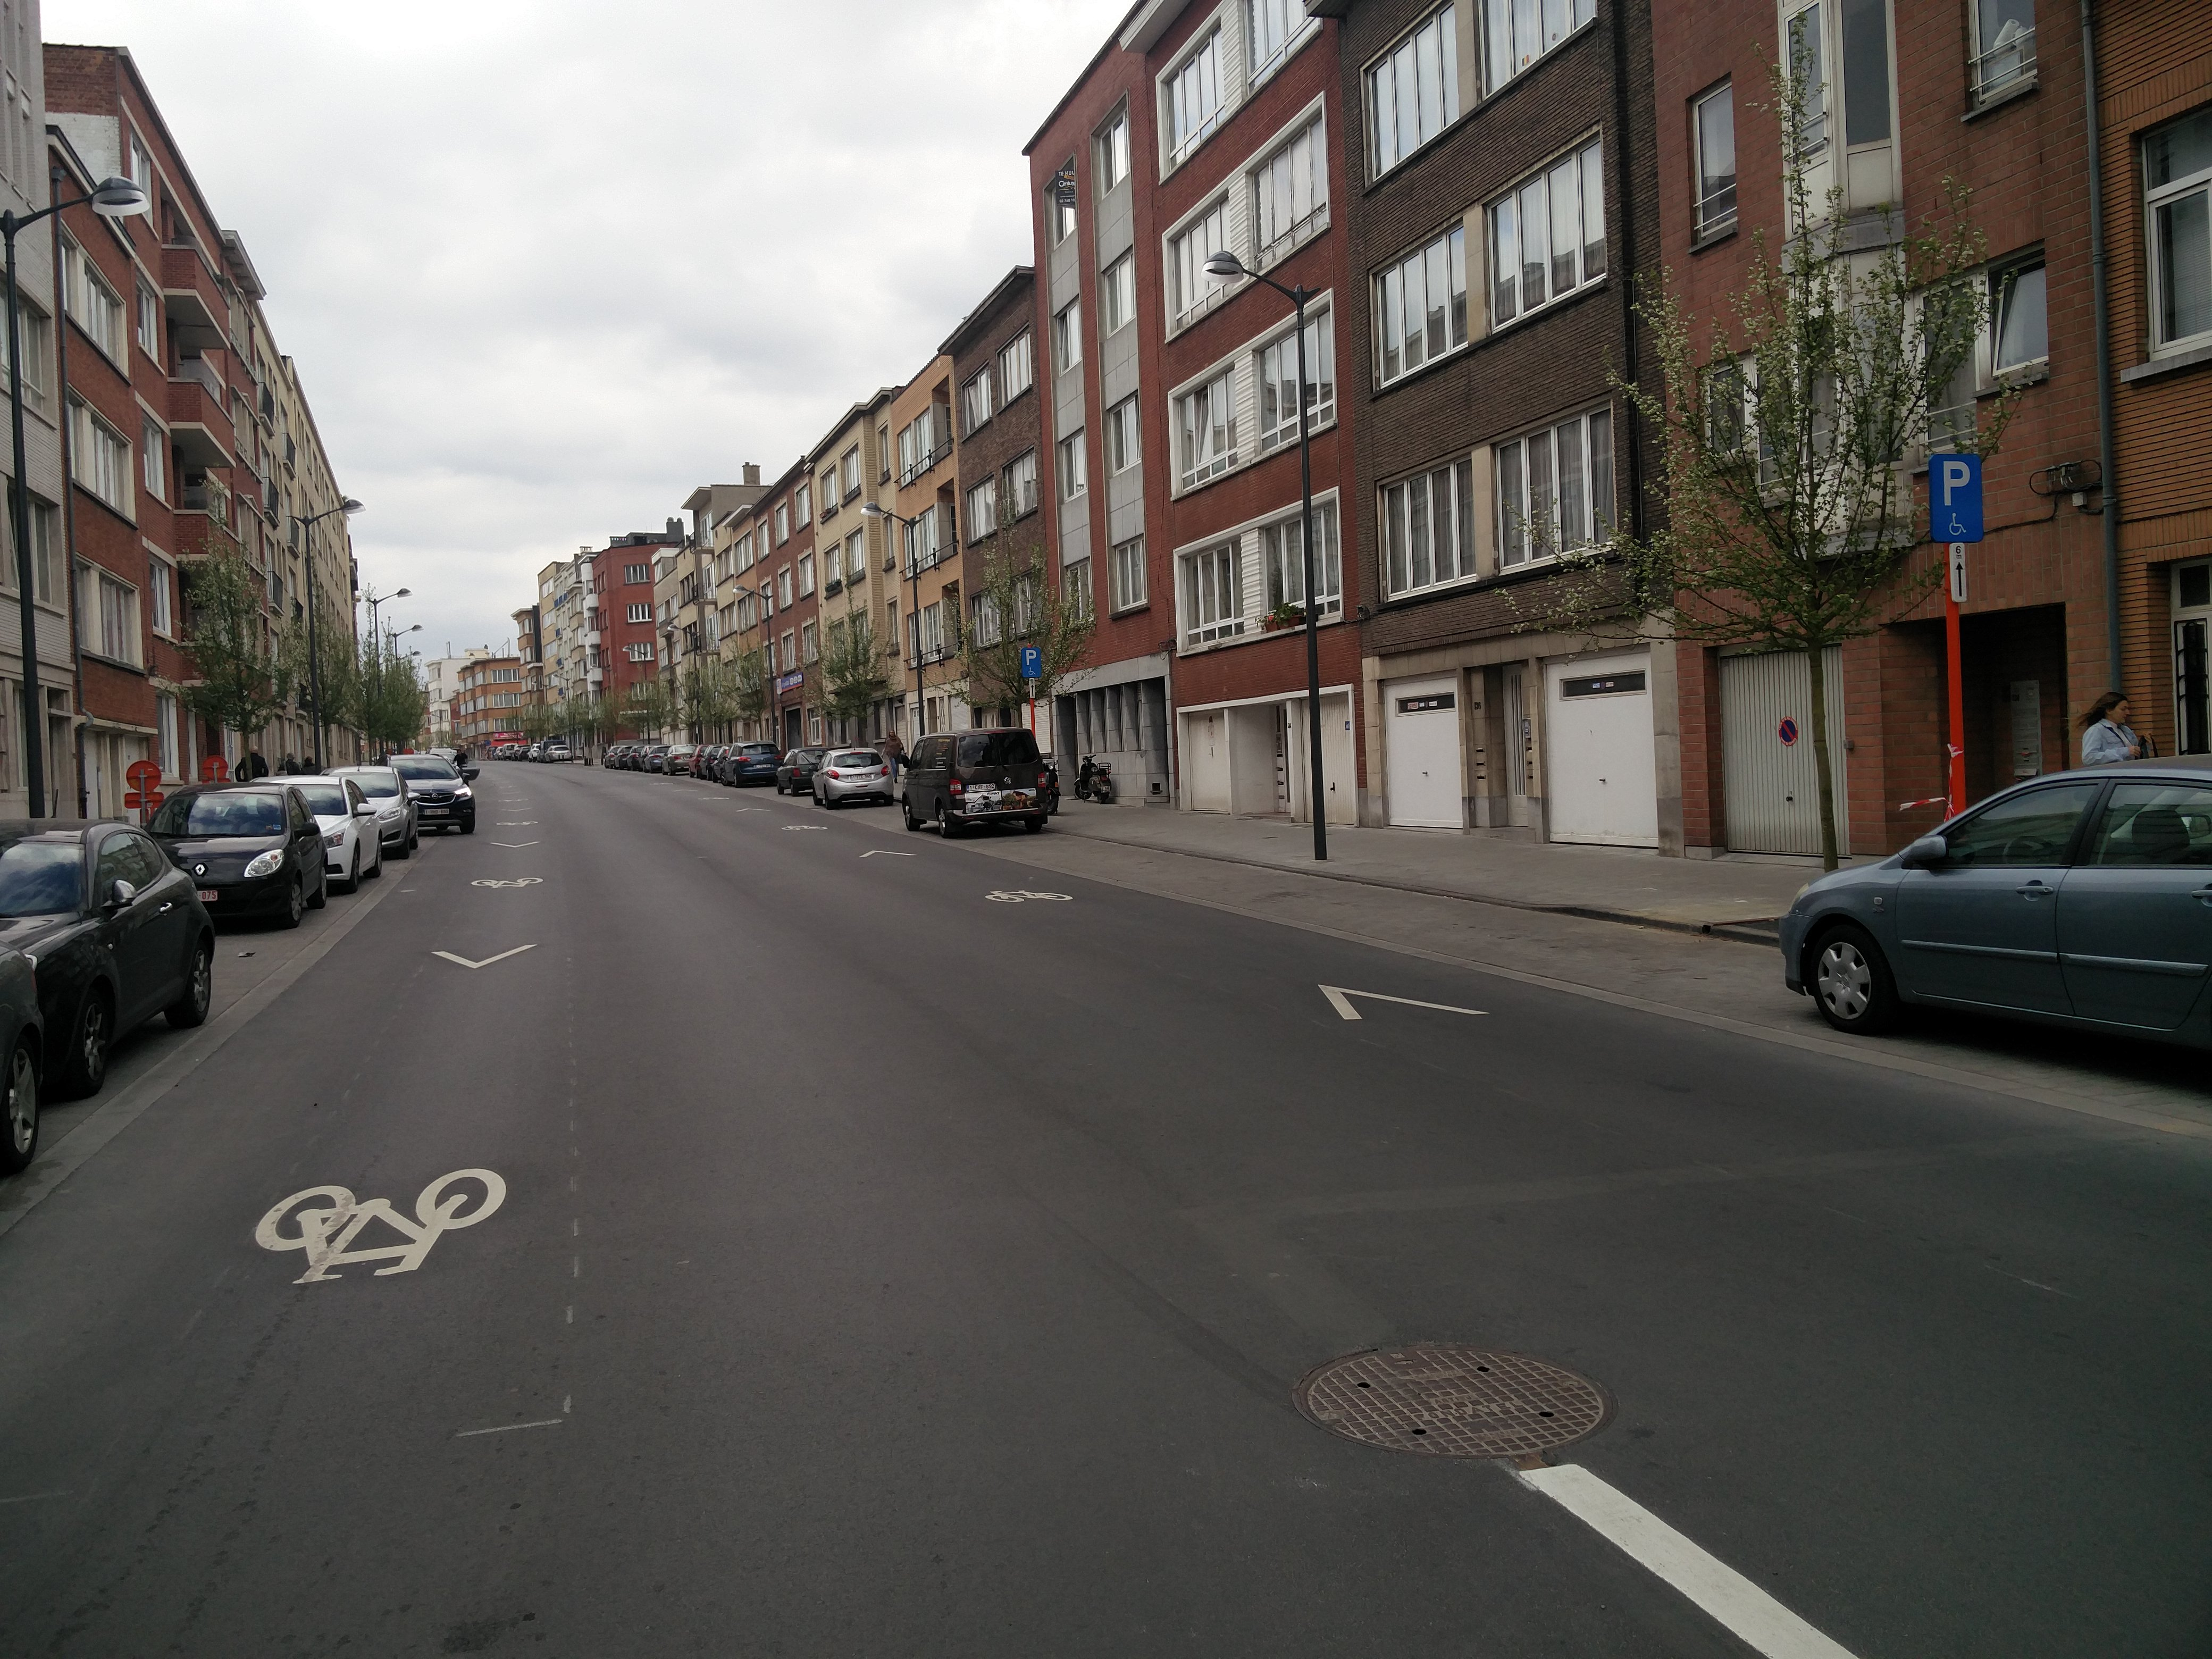
\includegraphics[keepaspectratio=true,width=\textwidth-2cm]{../images/ruexl.jpg}
\end{figure}



When connecting those two facts, a solution for the parking shortage arise and leads to a non-zero-sum game. Indeed, if the parking owner rent his space when he does not use it, he would earn money, and the driver would be able to rent the space thus finding a spot easily and he would have to pay anyway to park his car. It is assumed that the driver would have to pay as he would be in a situation where he struggle to find a spot, thus in a dense area, thus a location where the parking is charged.\\

This is ultimately a private parking short-term rent solution.

\subsection{Market Segment}
\bp has to offer its service in dense area. The application will offer its service only in Brussels at first.\\

The choice of focusing only on one region is based on the fact that the application will need network effects to be successful. Thus heavy initial promotion is needed. The goal is to implement the offer successfully in Brussels first and then explore other accurate locations. Offering the private parking short-term rent everywhere, including non-dense area, would have bad impact on the image of the application. Indeed, if a user sees that there is no availability in his neighbourhood, he is unlikely to use it again, although there was no availability in his neighbourhood because there was no need.\footnote{survey} \\

Choosing Brussels as the first city to implement the project is an appropriate choice. Indeed, Brussels is a leading city in Europe. The city is dense. There are 700 000 cars in movement at peak hours for 265 000 available spots.\cite{parkbx} The macro environment presented how Brussels is suitable for \bp. The \autoref{bxmap} present a map of the parking rules in Brussels\cite{parkbx} : \\

\begin{figure}[h]
\centering
\caption{Map of Brussels' regulated parking area}
\label{bxmap}
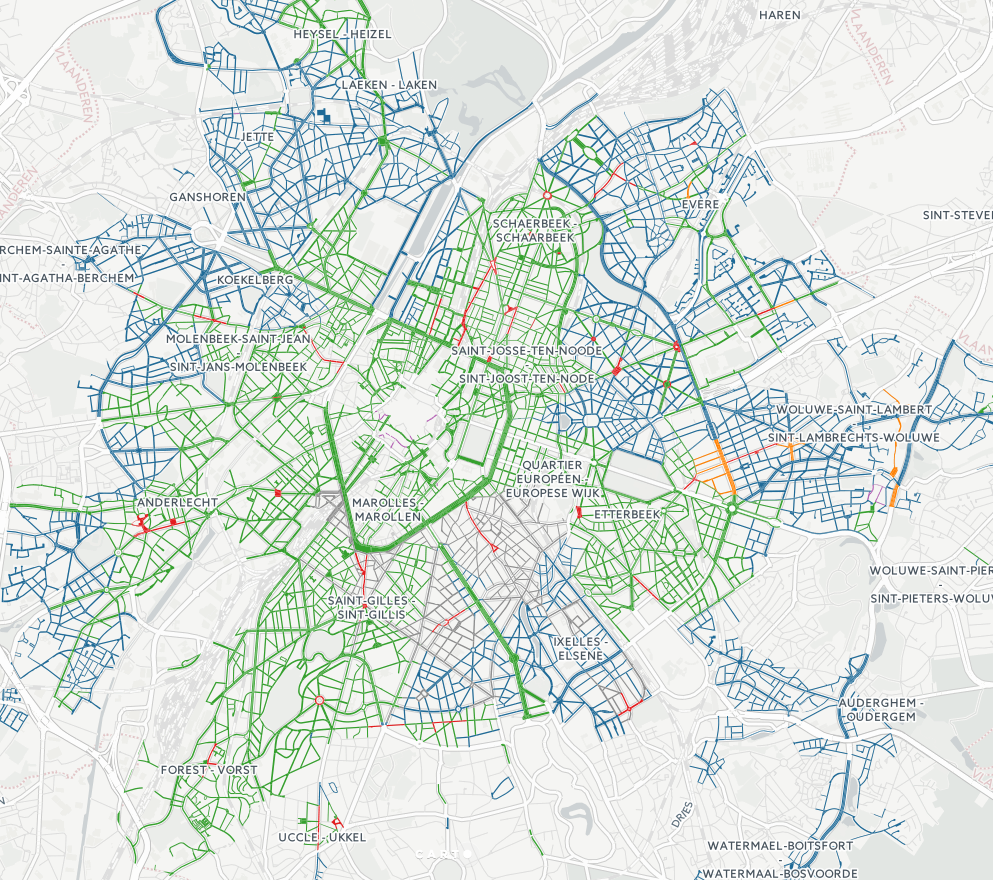
\includegraphics[keepaspectratio=true,width=\textwidth-2cm]{../images/bxpark.png}
\end{figure}


The blue area is free but for a length of 2 hours maximum and in the green, grey, orange and red ones, the driver needs to pay to park his car. The \autoref{bxfare} details the price and the maximum time in each zone.\\

\begin{table}[h]
\centering
\caption{Brussels's parking fare}
\label{bxfare}
\begin{tabular}{@{}lcccc@{}}
\cmidrule(l){2-5}
\textbf{}                                 & \textbf{Green} & \textbf{Grey} & \textbf{Orange} & \textbf{Red} \\ \midrule
\multicolumn{1}{l}{\textbf{Max}}        & /              & 4:30          & 2:00            & 2:00         \\ \midrule
\multicolumn{1}{l}{\textbf{0:30}}       & 0.50\euro{}           & 0.50\euro{}          & 0.50\euro{}            & 0.50\euro{}         \\ \midrule
\multicolumn{1}{l}{\textbf{1:00}}       & 1.00\euro{}           & 1.00\euro{}          & 1.00\euro{}            & 2.00\euro{}         \\ \midrule
\multicolumn{1}{l}{\textbf{1:30}}       & /              & /             & 2.00\euro{}            & 3.50\euro{}         \\ \midrule
\multicolumn{1}{l}{\textbf{2:00}}       & 3.00\euro{}           & 3.00\euro{}          & 3.00\euro{}            & 5.00\euro{}         \\ \midrule
\multicolumn{1}{l}{\textbf{3:00}}       & 4.50\euro{}           & 5.00\euro{}          & /               & /            \\ \midrule
\multicolumn{1}{l}{\textbf{4:00}}       & 6.00\euro{}           & 8.00\euro{}          & /               & /            \\ \midrule
\multicolumn{1}{l}{\textbf{4:30}}       & /              & 9.50\euro{}          & /               & /            \\ \midrule
\multicolumn{1}{l}{\textbf{Extra hour}} & 1.50\euro{}           & /             & /               & /            \\ \bottomrule
\end{tabular}
\end{table}

As a city with a heavily regulated parking policy, Brussels is the ideal candidate \bp to start its growth.

\subsection{Customer}
The service is based on two types of customer.\\

In the first place, there is the parking space renter. In order to be able to rent a parking spot, one would need to own a parking spot in Brussels. As the parking spot should be free at a recurring schedule in order to rent it consistently, employed people who do not work at home and use the car to go to their work place is an accurate person. One could assume that renting its spot would only attract not wealthy people but renting its spot is also an ecologist act.\footnote{survey} There is also benefit of renting a space if you are a user of the application on the other side as well. Indeed, there would be a bonus for space renters.\\

The second type of customer is the one willing to rent a place, the tenant. The people who might fall into that category need to use a car, whether it is owned or leased, in Brussels. They also need to have a smart phone and a mobile internet connection.\\
Whether this group of people will use the service or not is not related to any kind of wealth factor. Indeed, if a driver is looking for a spot and none are available for the period he desires, he cannot pay extra for a free spot, there are none available. If someone on the poor segment of the population is looking for a spot, he will want to find one and pay if needed as he is already in the location and going back home without completing the purpose of the ride is unlikely to be a better option.\\
More than just owning a smart phone, the typical user has to be aware that such technology exists. A person who knows and has used at least once \textit{Uber} would fall into such a category.

\subsection{Suppliers of the Industry}
The supply of the parking industry as a whole is parking spots. For \bp it is precisely private parking spots.\\
The particularity of the business model is that the supplier is also a customer. Indeed, it will be the owner of the parking spot that will have to register itself in the application and enter its parking spot in the system.

\subsection{Competitors}
\subsubsection{Parking Offer Comparison}
\label{poc}
Before analysing \bp 's competitors in its particular business model, it seems appropriate to compare the different parking offer and why \bp 's offer is relevant.\\

The \autoref{parkof} proposes a comparison of the different means available to a motorist to park his car. Commercial parking represents big parking lots owned by a private company, private long-term parking is a parking owned or rented on a monthly basis, finally private parking short term represent \bp 's offer.

\begin{table}[h]
\centering
\caption{Parking offer comparison}
\label{parkof}
\begin{adjustbox}{center}
\begin{tabular}{l|l|l|l|l|l|}
\cline{2-6}
\multirow{2}{*}{}                           & \multicolumn{2}{c|}{\textbf{Public Parking}\T\B}                                                      & \multicolumn{1}{c|}{\multirow{2}{*}{\textbf{\begin{tabular}[c]{@{}c@{}}Commercial\T\\ Parking\end{tabular}}}} & \multicolumn{1}{c|}{\multirow{2}{*}{\textbf{\begin{tabular}[c]{@{}c@{}}Private Parking\T\\ Long Term\end{tabular}}}} & \multicolumn{1}{c|}{\multirow{2}{*}{\textbf{\begin{tabular}[c]{@{}c@{}}Private Parking\T\\ Short Term\end{tabular}}}} \\ \cline{2-3}
                                            & \multicolumn{1}{c|}{\textbf{Free}} & \multicolumn{1}{c|}{\textbf{Regulated}\T\B}                      & \multicolumn{1}{c|}{}                                                                                       & \multicolumn{1}{c|}{}                                                                                              & \multicolumn{1}{c|}{}                                                                                               \\ \hline
\multicolumn{1}{|l|}{\textbf{Stay}}         & Very Short                         & Very Short                                                   & \begin{tabular}[c]{@{}l@{}}Short and\T\\ Long\B\end{tabular}                                                    & Long                                                                                                               & Short                                                                                                               \\ \hline
\multicolumn{1}{|l|}{\textbf{Price}}        & Free                               & \begin{tabular}[c]{@{}l@{}}Cheap to\T\\ Expensive\B\end{tabular} & Expensive                                                                                                   & Moderate                                                                                                           & Cheap                                                                                                               \\ \hline
\multicolumn{1}{|l|}{\textbf{Location}\T\B}     & Scarce                             & Frequent                                                     & Scarce                                                                                                      & Scarce                                                                                                             & Frequent                                                                                                            \\ \hline
\multicolumn{1}{|l|}{\textbf{Availability}\T\B} & High to Low                        & High to Low                                                  & High                                                                                                        & Low                                                                                                                & Moderate                                                                                                            \\ \hline
\multicolumn{1}{|l|}{\textbf{Speed}\T\B}        & Fast                               & Fast                                                         & Slow                                                                                                        & Fast                                                                                                               & Fast                                                                                                                \\ \hline
\end{tabular}
\end{adjustbox}
\end{table}

From this comparison, it appears clear that each mean has a different purpose. Public parking is clearly aimed at very short term stays. Public parking is not available all the time as the spots might all be used. Thus, if someone needs a short-term stay, he would use a commercial parking but this offer is scarce, usually parking lots are present only several key locations, as it can be seen in \autoref{pubparcmap}. Moreover they are expensive, information about the price can be found in \autoref{priceana}. The short term private parking thus makes sense as it should be available (once the product is settled) and cheaper than the original parking. To summarise, this option would offer very short-term stay cheaper or when there are no spots available and short-term stay when it is not possible through a public parking (e.g. blue zone, free but a stay of maximum 2 hours). Another advantage is that it is fast compared to a commercial parking. In the commercial parking there is all the ticket procedure and then you have to leave the parking which can take time.\\

\begin{figure}[h]
\centering
\caption{Map of Brussels's Public Parking Location\cite{pubparkmap}}
\label{pubparcmap}
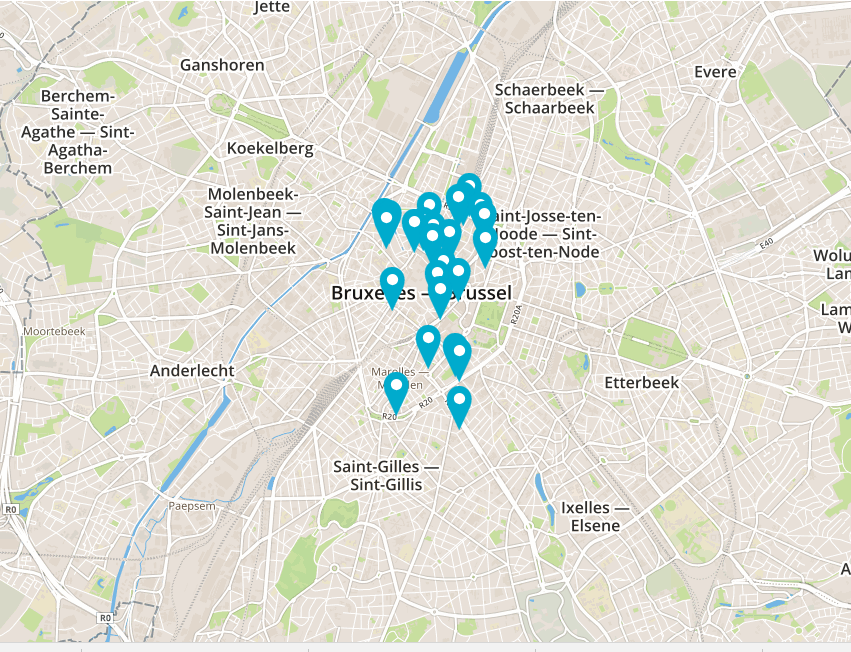
\includegraphics[keepaspectratio=true,width=\textwidth-2cm]{../images/publicpark.png}
\end{figure}

The long-term private parking has another purpose, to park the car for a long time or every day at the same spot. This parking option is not captured by \bp although having a private parking is not always possible and \bp could thus help the driver to find a place every day.

\subsubsection{Short Term Parking Offers}

Here is a list of selected competitors for \bp .

\begin{itemize}
\item \textbf{Parkopedia} offers to book a parking spot in parking lots online. It allows the user to compare price, check if there is availability and find an offer close to him. They have a strong presence, they have offers in 75 countries and 6308 cities. Although the business proposes a solution to finding a parking spot, the flaws identified in the previous section still holds, expensive, scarce location and time consuming.
\item \textbf{JustPark}, the services offer private parking rent for half an hour to a year and is available in almost all Europe. On average, the cost is less than 50\% of the parking alternative. It emphasis on popular location such as airports and stadiums. Any owner of a parking spot can add the spot to be rented and its availability. When renting a spot, there is a possibility to add a photo, a description and there is a comment system from previous renters. The owner of the parking selects the price per hour, day, week and month. The owner gets 80\% of what the user pays, the other 20\% goes to the application. Although the service could be used in all of Europe, it seems to be only used in the United Kingdom. Indeed, the application is very successful there but when looking for spots in Brussels, there is no parking available. The company was founded is 2006 in London. They raised venture capital from BMW i Ventures\cite{bmwi} and Index Venture.\cite{iven} They finally raised 1 million £ using crowdfunding, they achieved their target in just four days.\cite{crowd}
\item \textbf{ShareMyPark} has basically the same offer as \textit{JustPark} but it is available only in Brussels. The service has been created last year, in January 2016. The offer is rather weak, with only a hundred available spots in the city.\footnote{Based on research for a parking time of one hour in April 2017} On top of short-term parking, they also offer long-term and business parking.
\item \textbf{MyFlexiPark} is another similar service but this time available in all of Belgium. Launched in 2014.
\end{itemize}

There are other similar services as \textit{JustPark} but they are less successful. Thus \textit{JustPark} is the most successful service and \textit{ShareMyPark} and \textit{MyFlexiPark} are the only ones genuinely present in Brussels.\\
As \textit{ShareMyPark} and \textit{MyFlexiPark} have way less success than \textit{JustPark} overall, the market appears not to be captured in Brussels.\\
The \autoref{smp} shows that the offers in Brussels are way less known and followed than \textit{JustPark}, comforting the idea that Brussels's market is open.

\begin{table}[h]
\centering
\caption{Competitors' social media popularity in April 2017}
\label{smp}
\begin{tabular}{@{}lccc@{}}
\toprule
\textbf{}         & JustPark & ShareMyPark & MyFelxiPark \\ \midrule
\textbf{Twitter}  & 6 811    & 24          & 31          \\ \midrule
\textbf{Facebook} & 19 121   & 780         & 73          \\ \bottomrule
\end{tabular}
\end{table}

Another point is that \textit{JustPark} announces that they have 750 000 users\cite{jpu} and 25 000 spots available\cite{jpd} whereas \textit{ShareMyPark} and \textit{MyFlexiPark} do not make such claims. A potential explanation is that their user base is too low and would refrain people to register, as seeing the service as unsuccessful.



\subsection{Porter's Five Forces}
The following Porter's Five Forces analysis will focus on the short term private parking industry in Brussels. As this a rising industry the analysis has to be adapted.\\

\begin{itemize}
\item \textbf{Supplier Power} In this industry, the suppliers are the parking spot owner. They play a key role in the success of the business. Indeed, it is not possible to substitute their spot in any way, their offer is scarce. On the other hand, parking spot owner has a direct benefit in offering their parking spot as they would have a direct revenue in an easy and convenient way, almost no involvement from the owner is needed.\\
The owner of a parking spot alone cannot make the same offer as coordination services such as the one presented, thus there is close to no possibility of forward integration.\\
As the parking owner has a total control, the supplier power is high.
\item \textbf{Buyer Power} The buyers' behaviour depends upon the situation. Indeed, in neighbourhoods where it is easy to find a parking spot, the driver will not be willing to pay for a parking. On the other hand, in denser area, the driver knows that he will struggle to find a spot and potentially lose lots of time. In those areas, it is common for the driver to not even look for a parking spot but to go directly to a parking lot, e.g. next to a concert venue. Thus the buyer power depends on the context and would be low in dense area but high in others.\\
Overall, it is important to recall that the driver can always choose to look for another spot and is price sensitive.
\item \textbf{Threat of Entry} Potential entry in the industry is currently relatively high. Indeed, the market in Brussels is not captured yet and thus there is room for entry. However, if a service implements itself correctly, it would set a huge entry barrier as the network effects are very important for the service. To enter, two elements a required, an online platform and a user base. The platform can be built fairly easily but the user base construction is a complicate process.
\item \textbf{Threat of Substitutes} Two types of substitution can happen. Once in the car, the driver can use another means of parking. If there is available spots in the street, he can use them but as seen, in Brussels he would need to pay as well. The driver can also use a parking lot but this is not available everywhere and thus reduces its impact. This type of substitution threat is medium.\\
On the other hand, the motorist can choose to avoid using his car as a transport mean. Indeed, public transportation, bicycle and walking are other possibilities. In that case, the user would have no use of a parking spot. Although this is a serious threat, the transportation by car stays a very popular choice.
\item \textbf{Industry Rivalry} Finally, the intern competition of the industry is currently low in Brussels. Indeed the service is not well implemented and barely used thus the competition is very weak. The real competition that is currently taking place is the one of the most successful service. As analysed in the threat of entry, if a service succeed in imposing itself as the leading one and achieves  having a sufficient user base, then the network effect will make it the winner of the competition.
\end{itemize}

\chapter{Company and Product Description}

\bp will propose to the population of Brussels a fast, cheap and convenient way to park its car in the dense road of the city. Currently, similar online services exist but they struggle to find a user base, a crucial need of the service. Indeed, the success of the offer relies on network effects and once a service hit the critical mass, it will set a high entry barrier for other similar services. As opposed to the current offer \bp will place the incentive for parking owners to rent their driveway on the collectivism impact instead of the profit generation.\\

As opposed to the traditional way of parking \bp will be offering a way for drivers to find a place that is :
\begin{itemize}
\item \textbf{Fast}, by using the service, the driver will be guided to a spot. Indeed, a proposition of the nearest available locations will be displayed.
\item \textbf{Cheap}, the price of the parking will be 1\euro{} per hour.
\item \textbf{Convenient}, it will be possible for the driver to stay a long period of time, whereas the in-street parking is often limited in time. The billing will be directly link to a credit card thus making the payment process easier.
\end{itemize} 

Payment will be made online, through debit cards and credit cards. The renter will be able to withdraw his money from its location made through the service by bank transfer. The renter can also keep the money on its account for his personal use of the service, as a parking spot hunter.\\

As seen in the industry overview, the market target is quite large. Indeed, the service is useful for people who use their car in Brussels. The challenge is to build an offer of parking spot large enough, thus to attract enough parking owner on the service.

\section{Competitive Strategy}
\label{cst}
As explained in \autoref{poc}, \bp's offer is matching as demand that is currently not captured by the available parking service.\\

On the other, \bp has to attract the same customer that its competitors are targeting in Brussels. The angle of action is to focus on the collectivism impact of the application instead of the pure profit generation. It means that for someone to rent his driveway, its goal would be to be part of the service because he would like it to be available for him also in other locations.\\
This choice comes from two factors. Firstly, because of the apparent fail on focusing only on profit generation, as it seems to be the case for \textit{ShareMyPark} in Brussels. And secondly, because the profit generation is hardly possible. Indeed, let's assume that someone is working from 9 am to 5 pm during week days and is willing to lend his parking during that time. Per month, it would lead to a total of 160 hours of potential renting. Let's assume that the parking is rented all the time, at the same price as the in-street parking. In those ideal conditions, the renter would earn an extra 160\euro{}  per month. Although not negligible, the money generation is not enough for someone to make a living, for example. Moreover, as a parking owner, the renter is expected to have a certain level of lifestyle. To conclude, even in unlikely ideal conditions, the potential profit generation is low. But on the other hand, who has not been in a situation of wanting to park his car without obvious offer available ?\\
A survey conducted in the United States in 2016 showed that 80\% of online sellers says the extra money they earn is "nice to have but not essential"\cite{ospg}, reinforcing the idea that the profit generation is not the major of people present on online service with money generation.

To fulfil this aim, \bp will have major differentiation in its policy and its use:
\begin{itemize}
\item \textbf{Fixed Price} : the fares for the parking will be fixed. Indeed, in other services, whether it is  the successful \textit{JustPark} or \textit{ShareMyPark}, the renter chooses its price. This way of implementing the service is aligned with their emphasis on profit generation.\\
The fixed price will serve as a selling argument to attract customers. Our business will be able to guaranty that the price is half of the one in the street.
\item \textbf{Donations} : as \bp aims for sustainability and shared economy, it is aligned to give a part of its profit to association linked. As one of the incentive for driveway owner to rent them is sustainability and not profit generation, supporting charity will enhance it.
\end{itemize}

The ideal scenario would be that most of the transaction stays within the service, that renter uses their revenue only to rent other parking spot. Ultimately leading to a service where parking owner just exchange their driveways.

\subsection{Competitors Strategy Analysis}

\textit{JustPark} and \textit{ShareMyPark} are the two main competitors, this sub section has explaining why they are not successful in Brussels as goal.\\

Both competitor have the same offer and strategy, the renter sets his price. For \textit{JustPark}, it works in the UK and it is very successful. \textit{JustPark} is not targeting Brussels at the moment, they are currently aiming its promotion at Wales, specially Cardiff. On the other hand, \textit{ShareMyPark} have been targeting mainly Brussels for a year but the service is not successful. This observation lead to the following question : why is \textit{ShareMyPark} not successful in Brussels and subsequently why is \textit{JustPark} successful in the UK ?\\

The answer is that the market are not the same. In UK, finding a parking spot is even harder than in Brussels.\cite{londonpark} Which lead to a bigger demand, thus higher price and more benefit to rent a driveway.\\
Secondly, the Hofstede's individualism factor is higher in the UK than in Belgium, 89 versus 75.\cite{hukbe} Although the factor is quite high in Belgium, the one the UK is extremely high and thus may be one the explanation of the success of \textit{JustPark}.\\

To conclude, \textit{ShareMyPark} is believed to be not successful in Brussels because "set your price" policy. This strategy does not work in our market because the demand is not extreme enough. It thus struggle to find a user base and the profit generation incentive appear not to work.

\section{Reaching the Customer and Growth}
To reach the customers, three key elements will be used.\\

The first one is classic advertising. As the business is on-demand based, using technology and mobile phones, it seems appropriate to use online advertisements. Moreover, this type of advertisement allows our company to select our audience. The campaign could then focus people living or working in Brussels and owning a car. Social media advertisement is a good option as well because their user base is large, it would represent people who are already using mobile phone applications and thus more prone to use \bp's app.\\

The second promotion mean will be referring and word-to-mouth. Taking as an example successful campaign from \textit{Take Eat Easy}, \textit{Uber} and \textit{KeyTrade}, the idea is that if a user refer a new one, both of them receive an amount of credit. This lead to two positive effects, first one it incentive the user to refer their friend, thus increasing the user base. Second one is that the new user will be able to try the service for free, if he likes it he is likely to use again.\\

Thirdly, the last mean is targeted at parking owners. This promotion will be a physical one. The promotion itself will be a small paper aimed at a parking owner, offering them to put their poorly used driveway on the service. The idea is to hire students to go into the streets of Brussels by bike, and to slide the advertisement under the door of the garages that they cross.\\

Finally, as the service is based on collectivism, its popularity could be increased using local platform designed to promote sharing.

\subsection{Advantaging Driveway Owners}

The key component of \bp is the parking offer which is provided by driveway owners who are willing to rent it. As the owner will be part of our service in sustainability goal instead of profit generation, an issue could arise if he is not able to enjoy the offer of \bp. This could happen if there is way more user who do not rent driveway than actual renters.\\

The renter is compensated by an amount of money, but this money is expected to be reused within the application directly. Thus if the renter is constantly facing full spots, an issue will arise. \bp is designed to offer short term stays and thus it is unlikely that all the spot would be rented all the time. Moreover, the driveway owner does not need a spot all the time as he might have a parking at his workplace. On the other hand, if the renter needs a parking will working, thus frequently, \bp will give him an advantage over the regular user. The advantage is that regular user will be able to place a rent for a spot maximum 24 hours before the actual rent, whereas no such restriction will be placed on the renter. It thus allows the driveway owner to have a solid and regular parking option and it will not penalise the regular user for the first use of the application, which is sporadic short term parking.\\

The potential problem arose because once a user place a parking location, it would be annoying for him to remove it and impossible if he is already parked. As the driveway owner are the core of \bp, it is normal that they have an advantage over the regular user, otherwise a lack of offer could happen.

\section{Internal Analysis}
The business is not implemented yet but the following describes the aimed resources and capabilities of it.\\

As tangible resources, the software developed will be its core. Although software is not tangible, it is classified as so here because it is the key component of the business and will be a major investment of the business. There will be three declinations of it, a website, an Android application and an iOS application.\\

The intangible asset will be the reputation of the service and its user base. These two elements will have a key impact in the success of the service as it relies on reaching a critical user mass which will lead for the application to be useful. Opposed to the current offer in the Belgian market, \bp will focus on the collectivism effect of the service instead of only the potential profit generation for the parking spot owner. This part will be detailed in a following section.\footnote{link}\\

The human resource component will be quite low at the beginning. The equity holder possesses management and computer science skills which are sufficient to develop the business technically and strategically. However, maintenance and support will be needed so hiring will happen. Moreover, the promotion of the service will require other short-term hiring which will be described in the marketing plan.\footnote{link}\\

Finally, the capabilities of \bp will be its ease of use and access but mostly its capacity to establish itself as the only service to share parking spots and building user base. The last point relies on the network effect which is the key to succeeding in the industry.

\chapter{Marketing Plan}

\section{Relevant Market}
\label{rmar}
Brussels is the home of 1 175 173\cite{ciafb} inhabitants. The number of cars registered in Brussels in 2016 is 486 876.\cite{mtvr} Every day, there are also 350 000 commuters coming to Brussels.\cite{bxcommu} Which leads us to a total of 836 876 cars present in Brussels.\\
In 2015, in Brussels there was 266 498 garage, parking or roofed spot. Of all those spots, 55 314 were spots linked to a house, thus with an expected driveway.\cite{atpb}\\

In 2015, a survey about smart phone ownership tells us that, in France, 49\% of the population own a smart phone.\cite{spown} This statistic could help us to narrow down the potential market by assuming that the proportion should be roughly the same in Brussels. Reducing the market segment based on this percentage would be erroneous because our number of potential users is a selection of the population, the owners of car or parking. Thus it is more likely that this segment of the population own a smartphone.\\

The survey conducted concluded that college graduates, high-income and under 45 years old were the most likely to use on demand and shared services.\cite{airbnbuse} As our customer base is quite large, this group of people will be the first marketing target.

\section{Service}
\subsection{Parking Offer}
\bp is offering to the customer to rent a driveway. There are several extensions for this service :
\begin{itemize}
\item Renting personal garage
\item Offering to enterprise to rent their parking lot when empty, during the weekend for example
\item Having a premium system for some popular places next to stadium or concert venue
\item Offering a priority service to business where the employee could have some advantage to find a spot
\item Implementing co-operation with the commercial parking lot to add their offer to our
\end{itemize} 
The choice has been made to restrict the service to the driveway at first because, as explained, \bp relies on network effect. Thus it is important that the offer is clear and straightforward. By multiplying the service, the customer can be confused about what the purpose of the application is. Moreover, as the emphasis is on co-operation and collectivism, some of those examples are to be excluded because they are not aligned.

\subsection{Potential Collaboration}
Interesting synergies could arise from a collaboration between our parking rental offer and navigation application. Indeed, if a drive is using a GPS application to guide himself, it could be interesting for him to have several offers of parking near to his destination. As the duration of the journey is estimated by the application, it could even serve as a way to book a spot in advance and have more probability to find a spot that suits the driver.\\
Such services are offered by \textit{Google Maps} or \textit{Waze}. Those services are to be used from the smart phone and are on the leading edge of the navigation offer. Indeed, it takes into account the traffic of the journey and \textit{Waze} is even one step further, by allowing users to alert the other user of traffic trouble, such as a car in the emerging lane. \bp's offer would thus be an interesting addition to their service.\\
As those applications are already quite successful and powerful, it will be hard for our emerging service to be interesting to them in the first place. However, the option will be explored as the added value is more than just the sum of both services.\\

Another collaboration could from a partnership with car manufacturer. The goal would be to implement \bp as an application the dashboard of the car. The service would be the same but it would be available directly within the car's computer. As \bp is not well implemented, such a collaboration seems quite unlikely at first. On the other hand, if \bp becomes widely used, having it offered from the car might be a feature that customers would like and thus providing value to the car manufacturer as well.

\subsection{Branding and Positioning}

In order to be popular, the offer needs to differentiate itself in some way from the other offer available.\\

Regarding classic parking offer, \autoref{poc} presents a detailed comparison of the offers sand shows how \bp's proposition is differentiated. To recall, it is fast, convenient and cheap.\\

Now within the private parking rental segment, the main competitor in Brussels is \textit{ShareMyPark}. The main point of difference between the two offers is the suggested goal of renting a parking spot, full explanation can be found in \autoref{cst}. Briefly, the competitor emphasis on profit generation where \bp emphasis on collectivism.\\

The name of the offer is the first impact on the user mind and should thus reflect the value of the offer but at the same time be self-explanatory. The name \bp is designed to be aligned with those requirements. Indeed, the work park is the name, so it reflects in a straightforward way that the offer is about parking. Then, the prefix is "\textit{co}", which refers to collectivism, co-operation, collaboration. This prefix as two purposes. The first one is announcing that the offer is about working together toward a common goal, facilitating parking in Brussels. The second one is explaining that we will reach this goal by sharing our assets.\\
On top of that, in the French language, the prefix "\textit{co}" is used to denote sharing, for example \textit{covoiturage} means carpooling and could be translated to \textit{codriving}, \textit{colocation} means flatsharing and could be translated to \textit{corenting}. Finally, although it is not the main value, "\textit{co}" can lead a green image as it is close to "\textit{eco}" which refers to ecology.

\subsubsection{Positioning Statement}

\bp offers to the car drivers of Brussels a faster, cheaper and more convenient way to park their car than any other parking option. We are able to propose this offer by allowing citizens of Brussels to share their driveway between each other. Unlike other parking options, the price is low because the aim is not profit but making everyone's life easier by facilitating parking. The process will be fast and convenient thanks to the mobile application and geolocation. The parking owner will benefit from their rent by basically using the service for free. 

\section{Pricing}
\label{priceana}

As \bp's does not follow a profit generation aim for the renter, the goal is not to set a high price. Before going into detail, here is a comparison of the parking price in the competition.

\begin{itemize}
\item \textbf{In-street} : the \autoref{bxfare} shows the price of parking a car in Brussels. In the area where it is not free, the price is roughly \textbf{1\euro{} for the first hour and then 1.50\euro{} to 3\euro{} for the following}.
\item \textbf{Parking lot} : \textit{Interparking} owns 25 parking lots in Brussels. Their price goes from \textbf{1.30\euro{} per hour to 2.50\euro{}} depending on the area, with a large majority over 2\euro{}.\cite{interpk}
\item \textbf{MyflexiPark} : the following \autoref{fpprice} present the price per hour of the 56 available parking spot in Brussels in April 2017.

\begin{table}[h]
\centering
\caption{Price per hour and availability of parking spot on \textit{MyflexiPark}}
\label{fpprice}
\begin{adjustbox}{center}
\begin{tabular}{@{}lcccccccccc@{}}
\toprule
\textbf{Price}  & 0.50\euro{} & 0.90\euro{} & 1.00\euro{} & 1.50\euro{} & 1.75\euro{} & 2.00\euro{} & 3.50\euro{} & 4.00\euro{} & 5.00\euro{} & 10.00\euro{} \\ \midrule
\textbf{Availability} & 1           & 1           & 24          & 3           & 1           & 12          & 1           & 9           & 3           & 1            \\ \bottomrule
\end{tabular}
\end{adjustbox}
\end{table}

The most used prices are \textbf{1\euro{}, 2\euro{} and 4\euro{} per hour}.

\item \textbf{ShareMyPark} : the \autoref{smpprice} detail the availability of parking spots by a range of price per hour in Brussels in April 2017.

\begin{table}[h]
\centering
\caption{Range of price per hour and availability of parking spot on \textit{ShareMyPark}}
\label{smpprice}
\begin{adjustbox}{center}
\begin{tabular}{@{}lcccccccc@{}}
\toprule
\textbf{Price}       & $\leq$1.00\euro{} & $\leq$1.50\euro{} & $\leq$2.00\euro{} & $\leq$2.50\euro{} & $\leq$3.00\euro{} & $\leq$4.00\euro{} & $\leq$5.00\euro{} & >5.00\euro{} \\ \midrule
\textbf{Availability} & 3            & 11           & 65           & 27           & 3            & 4            & 10           & 3           \\\bottomrule
\end{tabular}
\end{adjustbox}
\end{table}

It is interesting to note that there is 49 spot at a rate of \textbf{2\euro{} per hour} and another 26 for \textbf{2.50\euro{} per hour}. Combined they represent 75 spot, which is more than 50\%.
\end{itemize}

The summary that can be drawn from this analysis is that the parking lot is the more expensive, \textit{MyflexiPark} has prices set close to the in-street parking and finally \textit{SharMyPark} is overall more expensive than in-street parking, especially for stays of one hour.\\

In the similar services proposed by \textit{ShareMyPark} and \textit{MyflexiPark}, the price is set by the owner of the parking. This lead to this diversity of price. If the application becomes popular, a price competition between the renter could emerge from this practice.\\

Following the differentiation point of \bp, the price will be set for the renter in our offer. The price is straightforward : \textbf{1\euro{} per hour} with a minimal stay of half an hour for 0.5\euro{}.\\
This rate is the same of the price to park a car in the street for the first hour. The first hour rate is selected because \bp's offer focuses on very short term and mid-term stay which are not available through in street parking, e.g. fours hours.\\
Having exactly the price of the in-street parking is a strong marketing claim for the user.\\

On the side of the parking owner, one may think that such a low price will not attract driveway owners as their revenue would be too low. However, the reason why someone would rent his park is not to earn money but to enrich the \bp's service as the renter would be a regular user as well. The money that the renter earns is not supposed to be withdrawn but reinvested to use the service on the other also, although the renter can get the money if he wishes. More information about the renter behavioural analysis can be found in \autoref{cst}.\\

In the same way as \textit{ShareMyPark}, \textit{MyflexiPark} and \textit{JustPark}, \bp will have a 20\% tax on every driveway location. This fare is present for the service to be sustainable and is sufficient enough.\footnote{link financial plan}\\

\subsection{Alternatives}

Other pricing strategies involved having a price of half the in street one. This lead to a price of 0.50\euro{} per hour. Although an attracting price, it is to low to be interesting. Beside financial stability that could be reach which such a price\footnote{to check}, it is expected to have several bad impact. The first one is that the parking owner who rent their driveway might think that they can directly pay instead of renting the driveway and use to money from the rent. Thus it would decrease an incentive to rent a driveway. The second one is that having such a low price can prevent the user from using the service. The idea behind is that it is too good to be true, it is so cheap that people think it is not sustainable.\\

A membership was also investigated. This pricing strategy is for the member to pay each month a fix price and then be able to use all the spot any time when available. This method might be interesting but it is not possible to implement it as a starting strategy since the parking offer is currently null. \bp could change its policy after having acquired a big enough offer but it seems inappropriate. First of all, when the offer will be present, it will mean that the user like to application as is, thus changing its operation is not interesting. And secondly, changing the policy or announcing that the policy will change after some tome will confuse the user base.\\

A dual pricing was analysed as well. The idea was to have different price whether the user of the application is renting a driveway or not. The price would be lower for the renter. This strategy would lead to a straightforward incentive for users to rent a driveway. This a good point. But in the current strategy, the renter is already rewarded by earning money from his rent. Another problem is that a renter would have different revenue from its spot as there is different price. This idea was dropped because it would make the service over complex with no new incentive.

\section{Distribution Plan}

As \bp offers a service, the distribution strategy is pretty straightforward. Driveway rental is planned to happen from the smart phone of the user, through an application, wherever he is. It is also possible to book a parking sport from the website application through a desktop computer. There are no intermediaries between, the service and the user. On the side of the renting a driveway, it is only possible in selected area where it is useful. The external analysis in \autoref{iechap} has presented Brussels and why this regional area is a relevant choice to implement \bp.

\section{Communication Plan}

As for every business, awareness is a key component of its success. A fortiori for \bp since network effect are heavily present. Thus the communication around our offer is crucial.\\
There are two different groups to target, the first one is composed of the driveway owner and the second of the car owner; in Brussels for both.\\
This section will present an integrated marketing communication strategy that will be implemented in order to inform our potential customer of our offer.\\
The communication around the car driver in Brussels will be aimed at college graduates, high-income and under 45 years old because it was presented in \autoref{rmar} as the segment of people who are the most likely to adopt our new service. Building the awareness of \bp for driveway owners will follow the same process but with a physical advertising extra. This emphasis on the renter is important because without renters there is no parking spot to be rented and thus the service we propose does not fulfil its aim. On the practical side, targeting a driveway owner physically is easy as it is not a hidden asset.

\subsection{Public Relationship and Events}
Brussels possesses a young and dynamic environment with several universities and several schools for superior studies. Several locations are known to be more frequented by younger people than other, those will be our target.\\
In order to attire driveway owner and driver from our target group, partnership with the popular event in Brussels is a good opportunity, the following is a selection of relevant events and what our partnership would be :

\begin{itemize}
\item \textbf{Apéro Urbain} : this is a recurring event in Brussels that takes every summer, from May to September, every Friday from 5 to 11:30 pm. The event consists of a party in with bars and DJ in an open-air localisation. The venues are popular places or park in Brussels. Their aim is : \textit{"Bring people at the same place to share a happy moment altogether"}.\cite{aperourbain} It can be seen on the picture available on the website that the population in those events fits our target. The audience is mostly 22 to 35 years old and involved in technology as the \textit{Facebook} page of the organisation has more than 50 000 followers (April 2017).\\
The collaboration aimed is a partnership that would allow the user to receive 10 hours of free parking on the application if they subscribe with a code present on the \textit{Facebook} event. The free offer represent a credit of 5\euro{} and as 20\% is deducted on renting as service costs, it represents 4\euro{}.\\
It is thus a form of sponsoring for the event as people might want to join by car, our service would help their community to find a parking and might thus bring more people.
\item \textbf{Student association ball} : in universities and high school, it is frequent that the student association of the school or of the faculty they belong to organise a ball. At the \textit{Université Libre de Bruxelles}, the most popular one is the one from the faculty of Architecture, Engineering and Business. In the academic year 2016-2017, 3400 people said that they would go on the event \textit{Facebook}. Those balls gathers current or former students from the faculty, student from other faculties or school. The population is thus composed of students or young workers.\\
The partnership proposed is having a photo booth at the venue. The guests could take a picture of themselves using type of \textit{photomaton}, and would then need to enter its email address to receive the picture. There would be a watermark promoting \bp. When sending the picture by email, a quick advertisement of our offer will be present.
\item \textbf{Couleur Café} : a music festival which takes place late June in Brussels. In 2017, the festival will last for three days, from June the 30th to July the 2nd. Couleur Café is focused on the world music and cultural event. The event manager said that they want to offer to the public a "\textit{mixing festive, solidary and musical}.\cite{rtbfcc} The event is interesting for our offer because the festival gather people from several segments. The festival is family-friendly and thus gather people with different age. As defined by the organisation, one of their aims is to promote solidarity, the public is thus interested in collectivism and sharing initiative such as the one proposed by \bp.\\
Here, the goal would be to deliver flyers within the festival and the queue, offering as well 10 hours of free parking on registering. Two stewards would be required to distribute the flyer but, moreover, present the service and discuss it with the guests.
\item \textbf{Repair Café} : a meeting where people with some repairing skills help each other to repair broken object. It can be a bicycle, clothing, electronics and more. Everything is free and based on volunteering. A repair café can be started anywhere. The \textit{French-speaking Belgian Network of Repair Café} has 22 repair café registered in Brussels.\cite{repair} The community attending those events is thus obviously into sharing and good use of personal possession, which makes them potential users of our application.\\
The idea is to attend several repair café and present \bp's offer. Then to discuss it with all the interest members.
\end{itemize}

A partnership with the \textbf{Réseau de Consommateurs Responsable}, which translates to \textit{Network of responsible consumers}, is a good way to present our offer to a user base interested in sharing and collective opportunities.\\
The Belgian association describe its mission as accompanying citizens who wish to exchange foods, objects and services in the aim of creating conviviality, minimise ecological impacts and support a more solidary economy.\cite{rcr}\\
The association thus promote every initiative going in its direction, such as Repair Café for example. Having \bp's offer registered on their website would not only bring awareness around the offer but also present clearly its collectivism value.

\subsection{Advertising}
To target the driver, our advertising will take place over social media platforms. The selected one is \textit{Facebook} as it is the most popular in Belgium.\cite{smstat} Moreover, \textit{Facebook} allows to place ads based on several information of its user, such has location, interest and age. If a user is interested, he can click on the ad and be directed to the website of \bp.\\

Physical advertising will take place as well, focused on the driveway owner. A team of students will be hired and their mission will be to place flyers presenting the offer under the garage door and into the mailbox linked to the garage. The student will need to own a bicycle to fulfil their mission and they will be sent in predetermined area. The flyer will also contain the 10 initial hours of free parking and an extra 10 hours if the user register its driveway on \bp.\\

The flyer will emphasis the sustainability and sharing values of \bp. It will explain that renting the spot is safe and there is a protection system for renters. The renter has full control of the availability of his spot. Finally, the profit donation from \bp will be clearly stated.

\subsection{Social Media}
88\% of consumers following a brand on social media feel that they are more informed about the company actuality and  78\% are stating that it allows them to know it better.\cite{sminfo} The goal of \bp presence on social media will be to \textbf{inform} its follower of its actuality , to \textbf{promote} by bringing awareness of its existence and \textbf{present} to the concept.\\
In order to fulfil those aims, \bp will be present on the following social media\footnote{usage statistics\cite{smusage}} :

\begin{itemize}
\item \textbf{Facebook} : 79\% of Belgian internet users own an account.\\Goal : \textbf{inform} and \textbf{promote}.\\
The presence on \textit{Facebook} will be a page that user can follow. The page will share content about how the service is evolving, its upcoming event and partnership and facts. Followers will then be informed. Their interest (\textit{follow)} and interaction will the page (\textit{likes}, \textit{shares)} will be seen by their network. 
\item \textbf{Twitter} : 14\% of Belgian internet users own an account.\\Goal : \textbf{inform} and \textbf{promote}.\\
The \textit{Twitter} accountof \bp will share content about the day-to-day life of the enterprise. New driveway available, promotion stories, ongoing process and present other sharing initiatives aligned with our values. The information available are thus closer to the company and more entertaining than the \textit{Facebook} ones. \textit{Twitter} also possesses a relaying option that user can perform to announce to their community that they like an account.
\item \textbf{YouTube} : 48\% of Belgian internet users own an account.\\Goal : \textbf{present}.\\
A presentation movie will be created to present \bp in a clear and pleasant way. This type of teaser will be uploaded to \textit{YouTube} as it is the most used video sharing platforms.
\item \textbf{Instagram} : 12\% of Belgian internet users own an account.\\Goal : \textbf{promote} and \textbf{present}.\\
Finally, the \textit{Instagram} account of \bp will deserve the purpose of presenting the value of the company. A selection on picture and quote about sharing, collectivism and ecology will be displayed on the social media.
\end{itemize}

Social media presence is not to be forgotten but, moreover, if it is implemented it should be done correctly. Indeed, there are several hidden rules about the use of each of them and not following them will make the company look bad. Number of posts per day, type of content, hour of posting and more are to be respected.\cite{smrules}

\subsection{Sales Promotion}
As network effect are important for \bp, so is the word-of-mouth marketing.\\
Users have an incentive to invite their friend to use the service as it makes the offer grow. In order to increase this incentive and specially to help them succeed, a referral program will be implemented. On registering, it will be possible to enter a referral code. If the new member does it, then he will have 10 hours of free parking and the user of which the code is as well. If the new member register a driveway, then he and the original user will get an extra 10 hours, thus 20 hours total.\\
The result is an incentive for users to promote \bp, free trial for new members which may lead to later use and thus growth of the business.\\

Several successful service companies used word to mouth marketing using referral program as a means. Indeed, \textit{Uber} fast development is partially due to its referral program.\cite{uberef}

\subsection{Service Design}
As \bp will be used by its community only through mobile phone applications and website, their design is a capital aspect of the business.\\

Both means of use will share the following attributes :
\begin{itemize}
\item \textbf{User-friendly} is the most important asset of the design. The service should be easy to use and straightforward to understand. What is the available functionalities should appear clearly. An action should be done in as few screens as possible.
\item \textbf{Fast} loading of the pages and close to no loading time will be implemented. The opening of the mobile application cannot take a long time as it will make its use unpleasant. The booking of a parking spot should not involve long operation time.
\item \textbf{Pretty} design is required for the service to be popular. The colour choice is important, as colour is linked to value. Colour combination as well, a colour palette will be respected. In the recent year, flat design emerged as the best one. The motto is \textit{to keep it simple}.
\item \textbf{Search Engine Optimisation} will have an impact on the growth of \bp and will thus be included in the creation of the website page name and so on.
\end{itemize}

\subsection{Direct Marketing}

Direct marketing will be used through a newsletter service. Users can subscribe to a mailing list from the website, application or on registering. People who used our photo booth service at events will also be included into the mailing list with an easy way to unsubscribe if they wish it.\\
The newsletter will be weekly and be mainly a gathering of the best post of the week from the different social media, with an incentive for the reader to follow \bp on social media.

\chapter{Operation and Team}

\section{Location}
The does not require a physical building at first.\\
The first part of the business implementation is building the website and the mobile phone application, then marketing will follow.\\

The software development will take place in the private apartment of the owner of the company. The apartment is located in the center of Brussels and is big enough for meetings and day-to-day work.\\

\section{Asset and Service Requirements}
This section describe the assets and services that \bp require in order to be functional.

\begin{itemize}
\item The core of the \bp's software, the back-end. The part of the software is where computation are done. The back-end is where the algorithms are and where the database is updated. On the other hand, the front-end it \textit{"the visible part of the iceberg"}, it is basically a view for the back-end. As application are more and more multi-platform, it is common to have several front-ends.

\item A web front-end, for user to access \bp's service through a computer.

\item An iOS front-end, for apple smart phone owner to be able to use \bp.

\item An Android front-end, in order to make \bp accessible through Android based smart phone, such as \textit{Samsung}, \textit{Huawei}, \textit{One Plus} ...

\item A hosting service, to install our back-end and thus make the front-end parts able to connect with it.
\end{itemize}

\section{The Team and Labour Force Requirements}
\subsection{Management Team and Equity Division}
The initial management team of \bp will be composed of two people. The crew will be formed by Simon Picard and Dan Martens. Both members are friends since 2011 and were involved in the same sutdent association which required management and organization skills. From this experience, it is known that collaboration between the two friends works well. On the other hand, their friendship might make their view homogeneous. In reality, they have quiet a different personality and complementary skills. The following present each members and describes its role within \bp.\\

\textbf{Simon Picard} is the founder and the CEO of \bp. He has studied computer science and successfully obtained its master degree in the discipline in 2016 at \textit{Université Libre de Bruxelles} in Brussels. He then pursued a Master in Management at \textit{Universidad Carlos III de Madrid} the next year. Simon is a pragmatic thinker. The CEO will be responsible for Strategy, Marketing, Operations, Human Ressources, Finance and Accounting.\\

\textbf{Dan Martens} is a partner and the CTO of \bp. He studied computer science as well but at the \textit{Institut Paul Lambin} in Brussels for his bachelor and he is now pursing a master degree at the \textit{Université Catholique de Louvain} at Louvain-La-Neuve. Dan has been involved in several IT project where he built web application and gain improved its practical knowledge. Dan is has a creative personality. The CTO will supervise the R\&D department, develop and maintain the software of the company. He will also take care of Customer Service and Support.\\

In the first part, both member will work on the development of the software together. Once functional, Dan will then be in charge of its future where Simon is going to dedicate himself for the promotion and expansion of \bp. The development will be happening during July and August 2017. Dan will not be involved in the promotion process because he will be working on his master thesis in order to graduate. Dan will thus work only if necessary on the maintenance of the application.\\

The equity division will be 75\% for Simon and 25\% for Dan. This division is the results of the following thinking. The initial success of \bp requires on two operations, its initial software development and its promotion afterwards. The two component are equally important. As Dan will be involved only in the initial development alongside with Simon, he would then be accountable for 25\% of \bp implementation. Simon will be the only one managing the promotion part and thus being accountable for 75\% of \bp implementation. Hence the 75-25 division.

\subsection{Employees}

Beside Dan Martens our CTO, the company will not have long term employee. On the other hand, \bp will require to hire for short periods, in order to pursue promotional event. Those have been presented in the previous the communication plan\footnote{link}. For those employee, the company will look for students. Those jobs are short term and thus suits student who look for some extra money for their month. On a financial basis, students do not pay taxes and thus the money we will have to spend is lower. Finally, our job involve sportive activity such as biking, or standing and walking for some time for flyering.

\section{Process}

\subsection{Account Creation}
A user need to create an account in order to use the application on which \bp relies. The account must be personal, one user must have one account and reversely.\\
In order to register, the user need to enter a pseudo and a password to access its account. In order to link one account to one person, the user must provide its first name and last name.\\
To avoid fraud, the account has to be linked to an email and a phone number. Those will have to be confirmed by entering a code on the application that was sent to them.\\
It is possible to link its account to \textit{Facebook}, it will be useful for extra feature described later in this section.\\

If the user intent to rent spot, he has to register the car with which he will. The car registration need the matriculation number, brand and color. The car will have a name, and several car can be registered on one account.

\subsection{Register a Driveway}
To register a driveway, the user must have an account. Then, the user goes into the driveway registering section. There it will ask the localisation the driveway. The user has the possibility to add a picture of the spot and a description. Those extra are useful to find where the spot exactly. For example, the description could be "the spot is the one in front of the red garage door".\\

Once the registration done, the user has to set when the spot is available. He thus accesses to a schedule where he enter the availabilities by half hour slots. He can set periodic availabilities such has "every Monday from 9 am to 3 pm" or specific ones such has "on April the 27th from 2 pm to 7 pm".\\

The renter can change the schedule whenever he wants to. The only time when cancellation is not possible is when the parking is rented and in use, the user has to wait for the end of the booking. On the other hand, if there is a reservation but it is not happening yet, the renter can cancel it and the future tenant will be warned.\\

The renter has to possibility to make his parking spot available only to user without strike. A user gets a strike when he stays longer than he is supposed to be.

\subsection{Rent a Spot}
To rent a parking spot, the has to be logged into to application through a previously registered account. The user then arrive an the view destined to rent a spot. This view is a map with a search bar for the location and time period entries. By default the time period is set to now until the next hour and the location is the one where the user if geolocalisation if available, center of Brussels other wise. The user can change all the setting of the search request. He then see on the map the available spots for the time slot and there is a list showing the spots in order of proximity of the location.\\

On the spot list, the user sees how many time it was already rented. If the user clicks on a spot on the list, a new panel opens with the picture of the spot, the description and the owner of the spot. The user has to click on a button to confirm the reservation. On booking, the user has to select with which car he is going to park.\\

Once booked, the user drives to the spot, parks his car and that's it. The user will receive an alert on his phone when the time to free the spots is approaching.

\subsection{Additional Features}
A leader board will be created where user will be able to see who rented the most a parking and which driving owner has rented its spot the most. The leader boards will be monthly or since \bp launch.\\
The phone contact will be scanned to create a friend list for the user. It will be possible to recognize users from phone number, email or facebook friendship. On the friend list, the user can see who has been renting spots.\\
If a user does not wish to show his statistic, he can hide them.\\

If a renter goes to his driveway and sees that it used whereas the spot is not rented, he can make a complaint. In order to make a complaint, the user has to take a picture of the car, enter the licence plate and link to which spot the infraction is.\\
The tenant will receive a strike and he will have to pay a fine to the parking owner. The fine is 25\euro{} and is fully received by the owner. 25\euro{} is the price of a fine in the street of Brussels for not paying the parking.\\
The user also receive a public strike, the parking owners can set their driveway non available to public strike holders. This strike stays public for one month. After that month, the users cannot know about the strike.\\
If a user has received three strikes, he is banned from \bp. Hence the registration through mobile phone and email, in order to make fraud more difficult.

\chapter{Critical Risks}

ShareMyPark success

JustPark Focus on Brussels

Fail to attract driveway owner

Over use of non driveway owner

Spot usurpation

Legal Issue

referral program exploit


\section{SWOT}

\chapter{Financial Plan}

\section{Estimated General Demand}

\subsection{Maximal User base}

\label{mubsec}

The maximal user base has been defined in the Marketing plan\footnote{link} and concluded that there is a total of 836 876 drivers that could use \bp and a maximum of 55 314 driveway to be rented in Brussels.\\

A survey lead in the United States reports to us that 11\% of the population has used a service similar to \textit{AirBnB} to stay overnight in a private residence.\cite{airbnbuse}\\
If someone has already been using a house-sharing service such as \textit{AirBnB}, it means that he knows about the offer and the sharing economy. As \bp is also about sharing a private property, a link can be drawn between the two services.\\

By combining the maximal amount of users and the percentage, we obtain that there would be \textbf{92 056} potential users of the service and \textbf{6 084} potential driveways to be rented. However, house-sharing services are aimed a people who travel on holiday. This segment is generally high-income. \bp is broader and would facilitate the life of poorer people. Thus the number of users could be even bigger but as explained in the previous chapter, the real challenge is to make Brussels's population adopt the service. At the end, this combination gives us a good starting idea of the demand.\\

Another way to estimate the demand is to extrapolate the user base of \textit{JustPark}. The competitor as a total of 750 000 user\cite{jpu}. The service is mainly utilised in London, a city with 8 673 713.\cite{ciafb} Thus 8,6\% of London's inhabitant are using \textit{JustPark}. So it can be said that 8,6\% of Brussels's population would use \bp. Leading this computation to a user base composed by 101 615 people.\\
This estimated demand is close to the one previously found, encouraging the idea that the estimation is plausible.\\

\subsection{Offer and Demand}

The typical driveway renter would be someone who works and his willing to rent its spot in the mean time. Thus, during work day he would rent his spot from 9am to 5pm, or for 8 hours. The demand is expected to be higher during those hours because the in street parking has to be paid at that time.\\

The worker segment could thus be renting their driveway for 8 hours, five days a week. The worker segment can be estimated by using the unemployment rate in Brussels which is 20.4\%.\cite{unemploybx} The number of driveway rented by a worker is thus 4 842 at full market captured. This part of the offer thus represent \textbf{774 720} hours of parking rental per month (4 842 * 4 weeks * 5 workday * 8 hours). Per driveway it lead to \textbf{160} hours per month.\\

Seasonality is expected to happen during the summer because it is the period where most worker are going in holiday.\footnote{proof} The worker in Belgium has a minimum of 20 free days per year.\cite{hdbe} By assuming that the worker uses 5 of his free day to go in holiday for a week, the parking rental offer during July and August can be adjusted.\cite{hdbe} The model proposed is that during one week of those month, the parking offer would be available for seven days straight. As it is unlikely that rental will happen at night, the number of ours per day during holiday will be 12. Finally there will be \textbf{987 768} hours of parking rental in July and August (4 842 * 3 weeks * 5 workday * 8 hours + 4 842 * 1 weeks * 7 holiday * 12 hours). Per driveway it lead to \textbf{204} hours per month.\\

The user base analysis lead to 15 users per driveway available. Assuming that the driveway available will be rented all the time is unrealistic.\\

In a survey conducted for this business plan, the following question was asked \textit{"On average, excluding weekends, during daytime : what is the proportion of the time where your car is parked in a spot that you have to pay for ? (i.e in a paid parking lot or in a chargeable spot in the street)"}. Surveyed people said they were living in a dense city such as Brussels and they are or used to drive a car. The resulting average percentage is \textbf{24,3\%}.\\

Assuming that the classic user and the driveway renters users will grow at the same rate, it lead to a full rent of the parking available. Indeed, the average user is paying 24,3\% of the time to park his car during daytime, weekday. There is 15 classic user per driveway available. Thus it means that it would require only four user to fulfil the offer. With 15 users per driveway, it can safely be assumed that the parking option will be totally used. This analysis leads to a occupancy rate of 100\%. However, inefficiencies will arise, it is unlikely that users will be able to switch instantly in parking a spot. Thus the occupancy rate will be decreased to \textbf{90\%}.

\section{Cost of Marketing}

The physical advertising through flyers under garage doors will be made by student riding bicycle. Excluding the high speed lanes, there is 1 983,5 km of road in Brussels.\cite{mtvr} The speed when travelling by bike can be as high as 30 km/h but taking into account that the road network is not a straight line and that the employee will have to constantly go off of his bike in order the distribute the flyer, an 7 km/h pace is more realistic. It means that job will require 283 hours to completed. As the job require physical effort, a 10 \euro{} per hour salary will be offered. The cost of this operation will thus be \textbf{2 830 \euro{}}.\\

The average cost per thousand of impression for a \textit{Facebook} ad is 7,29\$.\cite{fbad} As our customer segment is quite small because it is only people living in Brussels, a thousand of view per day is as satisfying start. Thus the budget per day is 7,29\$, hence the budget per month 204,12\$, or \textbf{186,61\euro{}}.\footnote{Rate of USD 1 = EUR 0.9142 accessed on 09/05/2017, Eurpean Central Bank. This rate will be reused for the following conversions.}\\

The photo booth at the student ball requires a touch screen, a camera and small computing unit, also known as a micro processor. The \autoref{pbcom} shows the component and their prices. The total component price is 127,70\$ and 50\$ have to be added to capture the price of cables and wood to create the box holding everything. At the event, a student has to be hired for 6 hours to set the booth at the event and invite guest to take a picture. A classic wage of 10\euro{} per hour is expected. Thus, the building price is 177,70\$ or \textbf{162,45\euro{}} and the cost for the employee at the event is \textbf{60\euro{}}.\\

\begin{table}[h]
\centering
\caption{Photo booth component}
\label{pbcom}
\begin{tabular}{|l|c|c|}
\hline
\textbf{Name}   & \textbf{Price} & \textbf{Reference} \\ \hline
Monitor         & 80,00\$         & \cite{abmon}    \\ \hline
Camera          & 14,70\$         & \cite{abcam}     \\ \hline
Micro-processor & 33,00\$         & \cite{abmc}     \\ \hline
\end{tabular}
\end{table}

The partnership with Apero Urbain assume a free offer to the guests. The offer is 10 hours of free parking, thus the equivalent of 10\euro{}. As \bp takes 20\% as a fee, it represents a cost of 8\euro{} per new user. The \textit{Facebook} event from the 2016 edition gathered 3 000 users, based on there attendance on the event.\cite{fbau} Basically, the promotion whenever a desired amount of user registered and used the promotion. There is around 16 event per year with the same attendance range. Thus, assuming that at least 1 000 person would register is realistic. Those 1 000 registration would thus cost \textbf{8 000\euro{}}.\\


The promotion at Couleur Cafe festival is flyering and promoting \bp. Two steward are to be hired, one again student are targeted for the position. The flyring would start at 8 pm and last for four hours. The price to hire the employee at a 10\euro{} per hour rate is 80\euro{}, as the festival last three days, it would cost a total of 240\euro{}. As the promotion of 10 hours of parking is present as well, its cost has to be taken into consideration. There will be 20 000 quest per day in the 2017 edition. By assuming that 1\% of the guest are interested, 200 person would register for the application per day. Hence a total 600 registrations for \textbf{5 040\euro{}}.\\

The promotion at the \textit{Repair Café} and the collaboration with \textit{Réseau de Consommateurs Respondable} will be done by Simon Picard, as part of its spoke person responsibilities.\\

The community manager job will be held by Simon Picard, as part of his daily duties.\\

Finally, the referral promotion grants 10 hours of free parking to the inviter and the new user. It sums to 20\euro{} and \textbf{16\euro{}} after removing \bp's fee. During the growth stage, a large portion of the new user are expected to come from this promotion. The promotion will stop when the critical user mass is reached, this number will be analysed in the following section.

\section{User Base Growth}
\bp is revenues and expense are highly depend on the number of user it posses. Indeed, the server load, the number of referrals and the actual number of hour of parking rented depends on them.

In order to evaluate it, a contagion model will be used. A contagion model comes form the epidemiology field. It has already been used to analyse optimal advertising policies in the late 70'.\cite{sethi1979optimal} A suggestion of use of the model to estimate the user growth requires three data. Those are the \textbf{initial user base}, the \textbf{total population} and the \textbf{propagation rate}.\cite{cmep}\\

The total population has been estimated to be 92 056 in \autoref{mubsec}. The reach of the marketing campaign has been assessed to be 1 600. However, it is unlikely that all the registration will lead to regular user. Four of those registration out of ten will be kept as regular users. Finally the propagation rate can be computed by assessing how many people are required for a new person to start using \bp each month. If the propagation rate is 33\%, it means that each month a new person starts using for every three people already using.\\

The \autoref{ugp} shows a user base growth with a total population of 92 056, an initial user base of 640 and a contagion rate of 10\%. In this model, more than 90\% of the market is reached in 6 years and full population is reach in 12 years.\\

\begin{figure}[h]
\centering
\caption{User base growth projection. Population = 92 056; Initial users = 640; Contagion rate = 10\%}
\label{ugp}
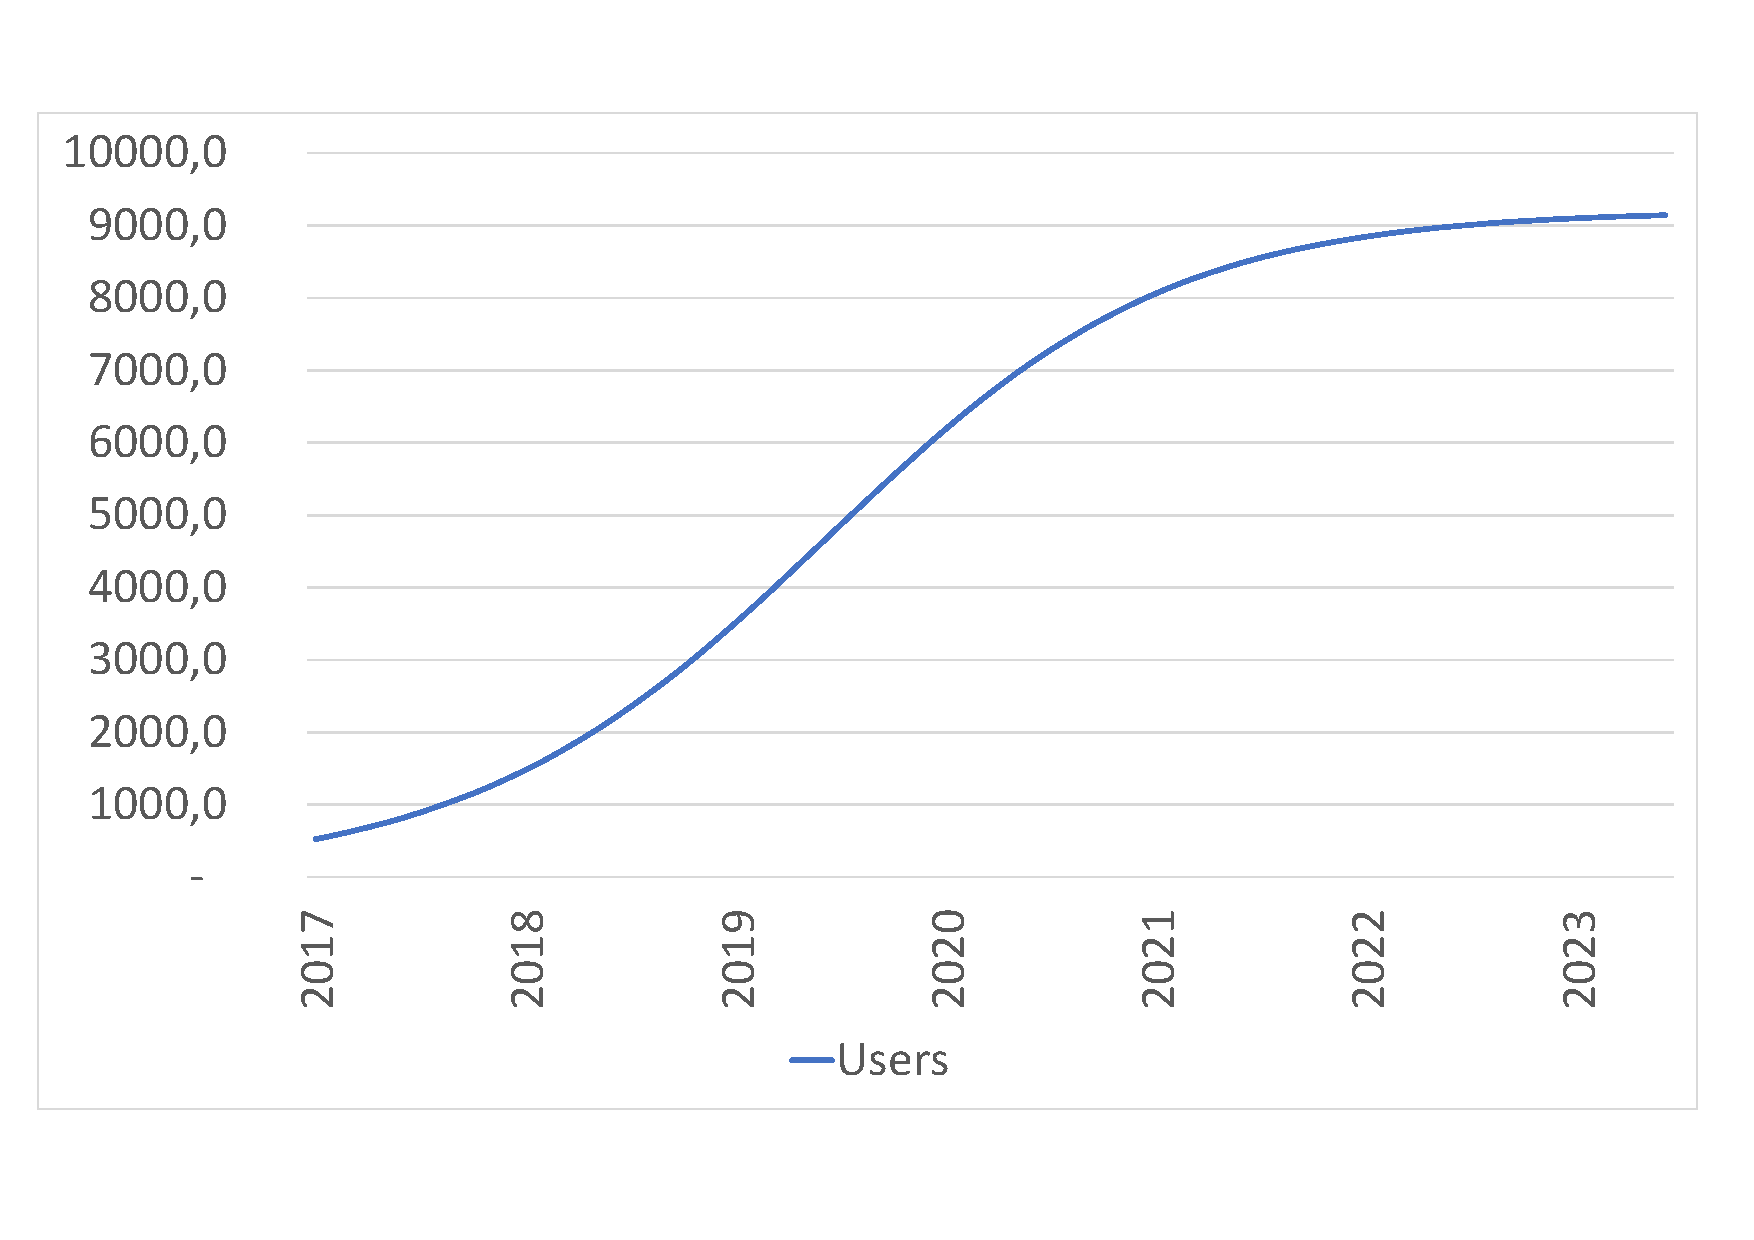
\includegraphics[keepaspectratio=true,width=\textwidth-2cm]{../graph/usergrowth.pdf}
\end{figure}

The latter inputs will be used for the following financial analysis as they appear quite realistic. However, those variable are crucial for the computation and will thus be part of a sensitive analysis.


\section{Cost of Operations}
There is only one operating cost in this business model and it is the rent of a server. Estimating the cost of the server is not an easy task because it depends on the load on it, which itself depends on the number of user and the architecture of the software.\\

The choice is to use a server provided by Amazon which is easy to scale. Basically, the server can be built as the customer which, with different services and power. The service that will be used is \textit{Amazon Elastic Beanstalk}. After on-line research and discussions with a web app developer, it has been analysed that the \textit{Large Web App} example on the \textit{Amazon Web Service Fee Calculator} could represent a server that would be suitable for a service with 50 000 simultaneous users and that a linear extrapolation of the monthly price with the number of user is relistic.\cite{itwlois}\cite{qaws}\cite{hsaws}\\

The price of a server suitable for 50 000 users is 893.29\$ per month.\cite{awsclwa} In after conversion it leads to 816,59\euro{}. Thus, the price to sustain 5 000 users is 81.66\euro{} per month.\\

After the development of the application, Simon Picard will be in charge of the marketing, day to day operations and maintenance. He will work full time for \bp and will receive the minimum wage which is \textbf{1 501,82\euro{}} per month.\cite{eurostatmw}\\


\section{Sale Forecast}

The sale forecast depends on the growth of the user base, the offer and the demand. Those factor have been analysed in previous section. Basically, the revenue are generated by the rents of the driveway, \bp takes a fee of 20\% on each rent. The price per hour is 1\euro{}, the company thus earns 0.2\euro{} per hour rent.\\

The process to estimate the revenue is the following :
\begin{enumerate}
\item Get number of driveway
\item Get offer by multiplying number of driveway per average number of rent per month
\item Get number of hour rented by discounting the offer by the occupancy rate
\item Get revenue by multiplying the number of hour rented by the fee
\end{enumerate}

Basic computations lead to an expected revenue per month, as shown in \autoref{ery13} for year 1 to 3. The detail of the computation and data can be found in appendix.\footnote{link}\\

\begin{figure}[h]
\centering
\caption{Expected revenue per month year 1-3}
\label{ery13}
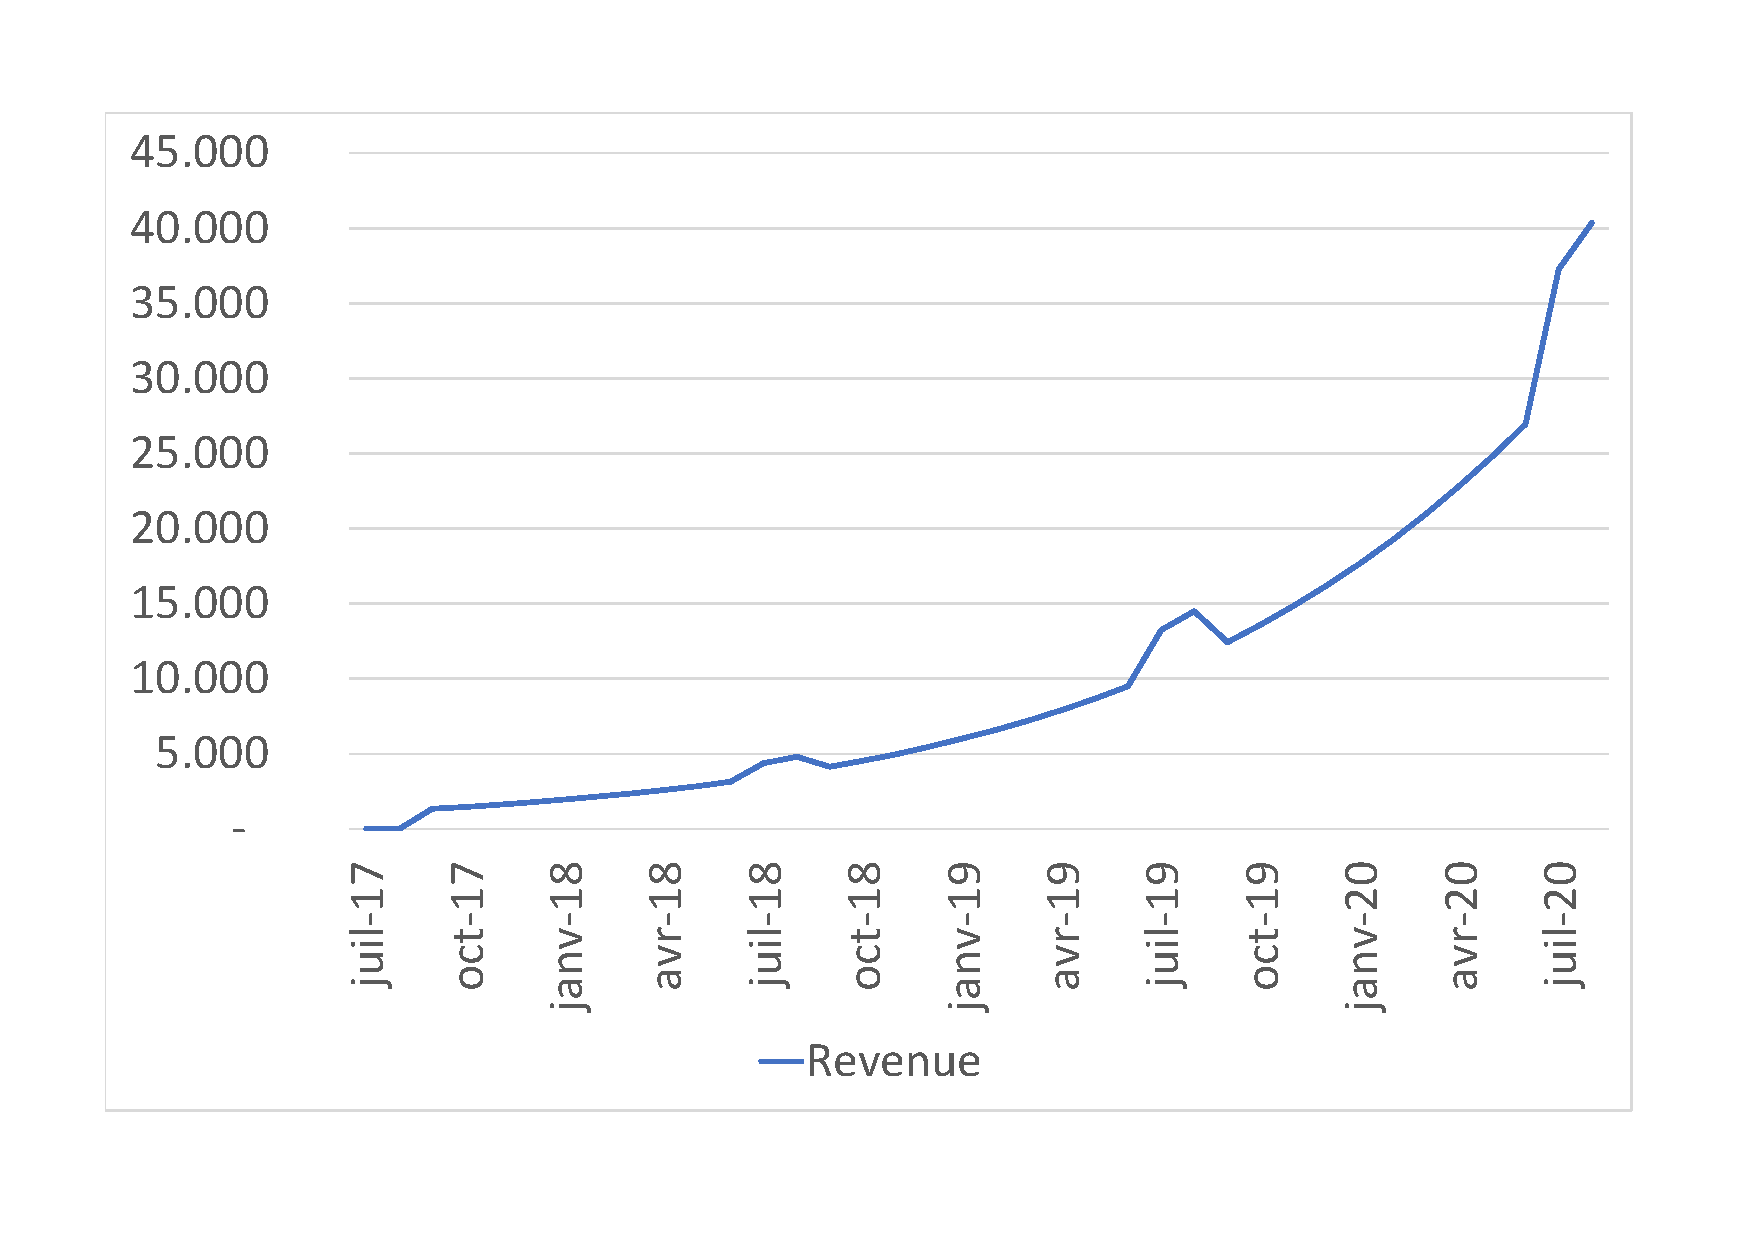
\includegraphics[keepaspectratio=true,width=\textwidth-2cm]{../graph/expectedrev.pdf}
\end{figure}

In summer, the seasonality appears clearly.

\section{Expenses}
This section asses the expense per month base on the previously analysed cost of marketing and operations.\\

The recurring monthly expenses of the service are formed by the wages and ad cost, which are fixed. On top of that, the referral program is to be taken into account. Each new user cost 16\euro{}. The server rent has a minimal price of 81.66\euro{} per month and once the user base becomes bigger than 500, the price is to be correlated as explained in the cost of operation.\\


The depreciation of the software is to be take into account as well. To fulfil its development, it will require two month of work from two computer scientist as assessed in previous chapter. The average monthly salary of IT specialist in Belgium is 4 704\euro{}.\cite{avslinf} The software is thus valued at four time this amount : \textbf{18 816\euro{}}. As the development world move fast, the software is expected to be outdated after three year. A linear depreciation will be used and will represent the cost of hiring Dan Martens to update the software when necessary.\\


The \autoref{eey13} present a graph of the monthly recurring expense of \bp for the three first year.

\begin{figure}[h]
\centering
\caption{Expected recurring expenses per month year 1-3}
\label{eey13}
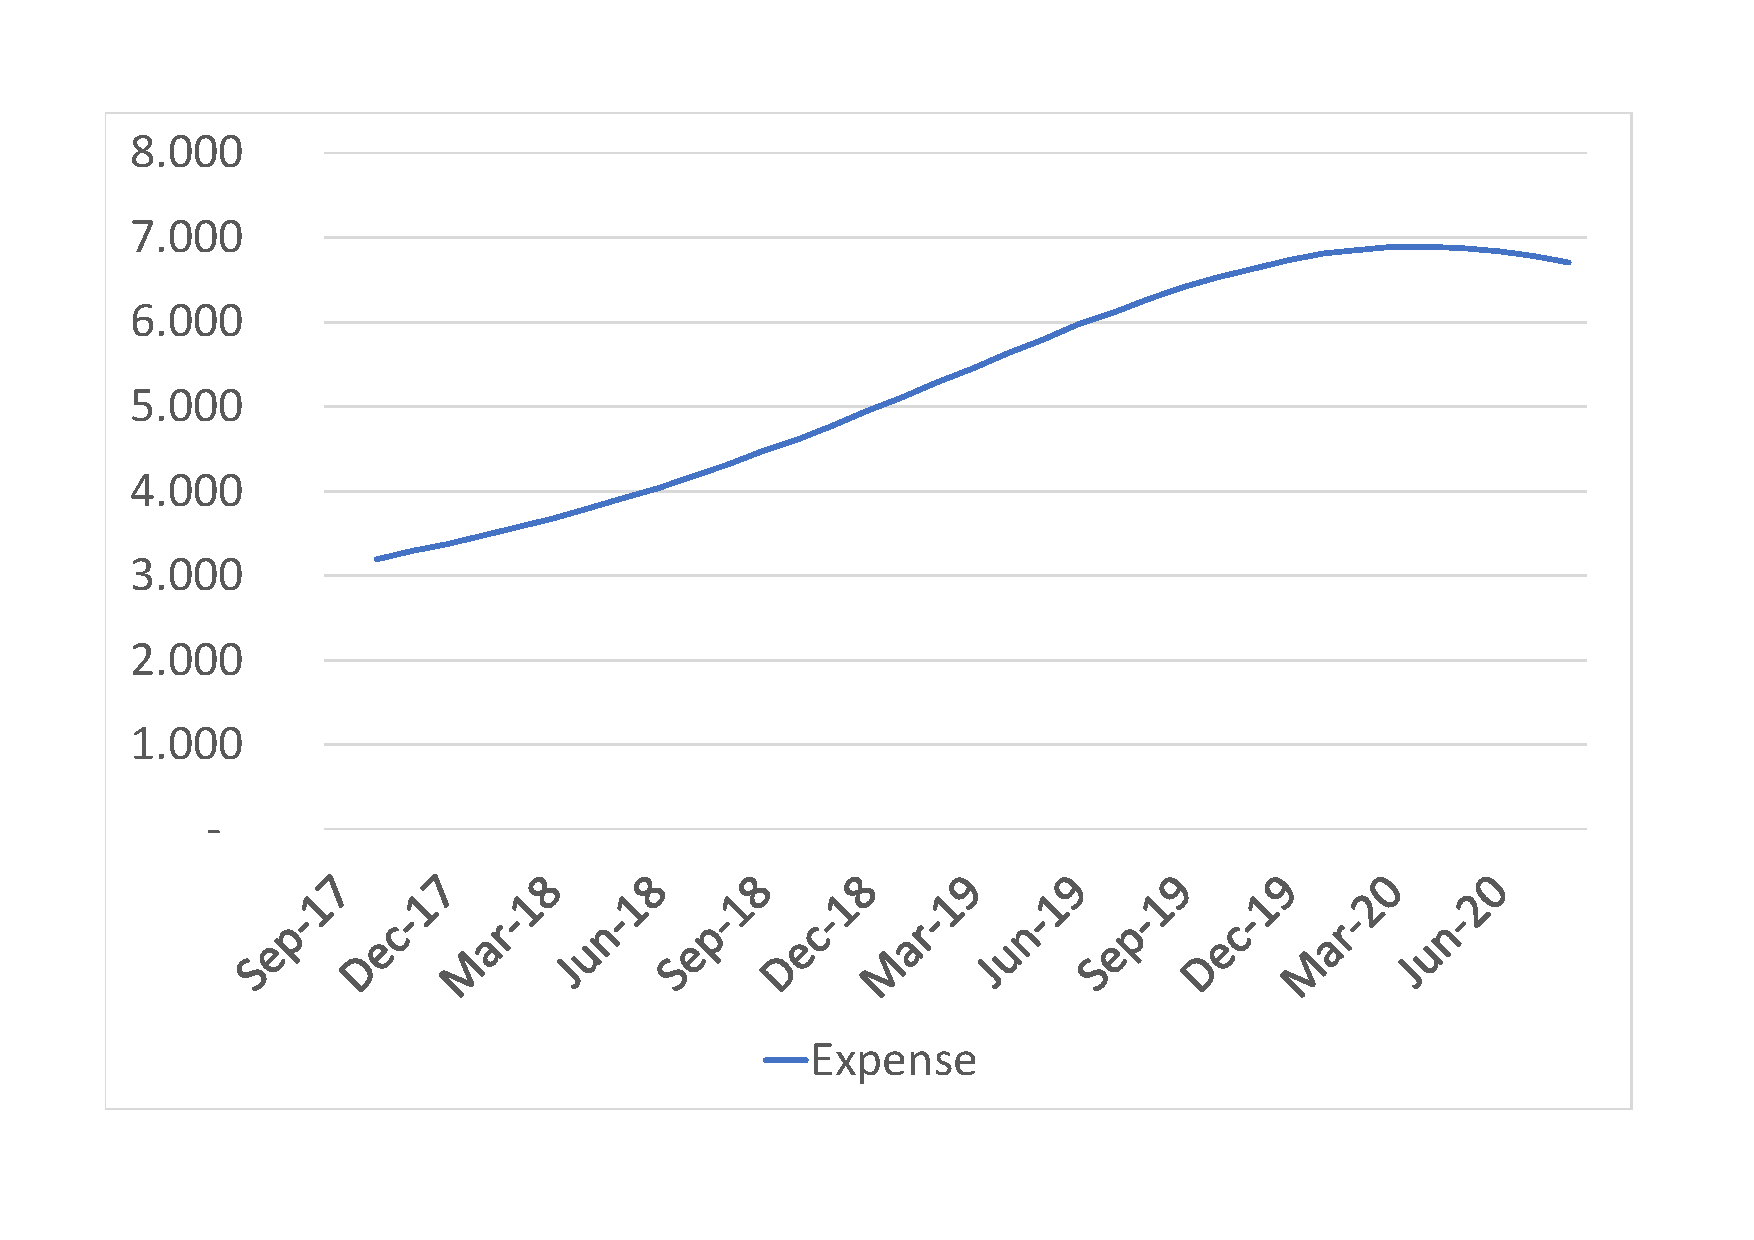
\includegraphics[keepaspectratio=true,width=\textwidth-2cm]{../graph/expectedexp.pdf}
\end{figure}

On top of those recurring cost, marketing operation have to be included.

\section{Income Statement}

\section{Cash Flow Statement}

\section{Balance Sheet}

\section{Sensitivity Analysis}

\begin{figure}[h]
\centering
\caption{Sensitivity Analysis}
\label{eey13}
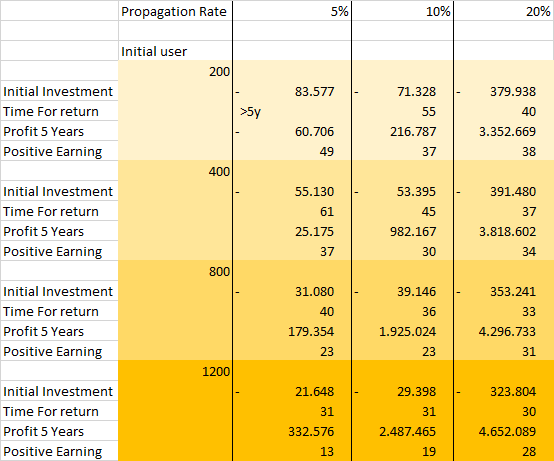
\includegraphics[keepaspectratio=true,width=\textwidth-2cm]{../images/sensitivity.png}
\end{figure}

\section{Funding}


\appendix

\chapter{Survey}
\begin{itemize}
\item Are driving a car frequently (i.e once a week or more)
\item Do you live in Brussels
\item Do you own a garage with a personal driveway
\item Do you own a smart phone
\item Do you usually struggle to find a parking spot in street?
\item On average, during daytime, what is the portion of the time where your car is parked in the street or in a paid paring lot ?
\item Would you be willing to let other people park in your driveway when you do not need it if you could yourself park your car in other driveway when they are available ? Important, imagine that your driveway will always be available when you need it. (If you do not own a driveway, assume you do to answer)
\end{itemize}

%\bibliographystyle{plain}
%\bibliography{./reference/bibliography}
%\printbibliography

\defbibheading{bibliography}[\bibname]
%\markboth{#1}{#1}}


\chapter{Bibliography}

\defbibheading{b}{\section{Books}}
\defbibheading{i}{\section{Internet}}
\printbibliography[title={Article references},type=article]
\pagebreak

\printbibliography[title={Other references},type=misc]

\chapter{Income Statement}
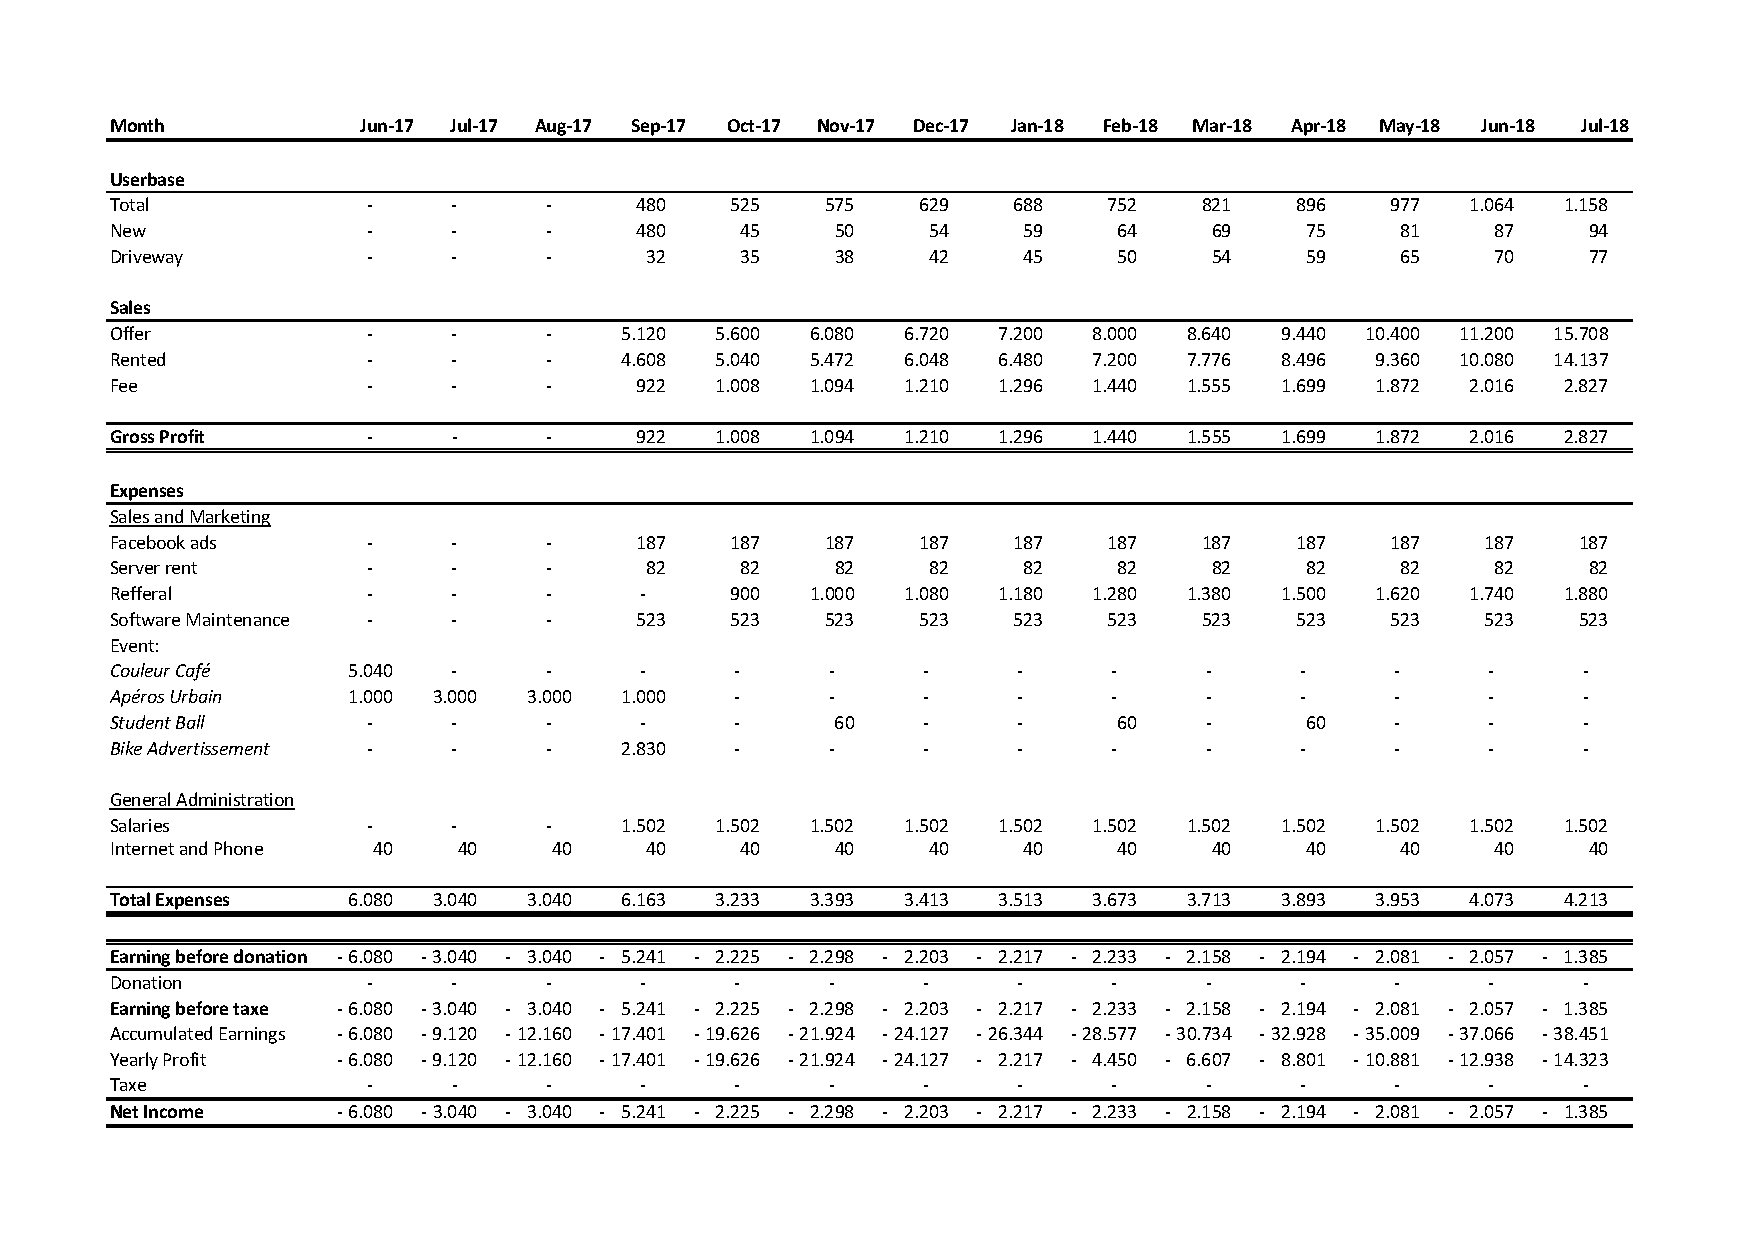
\includepdf[pages={1,2,3},landscape=true]{../sheets/income.pdf}

\chapter{Cash Flow Statement}
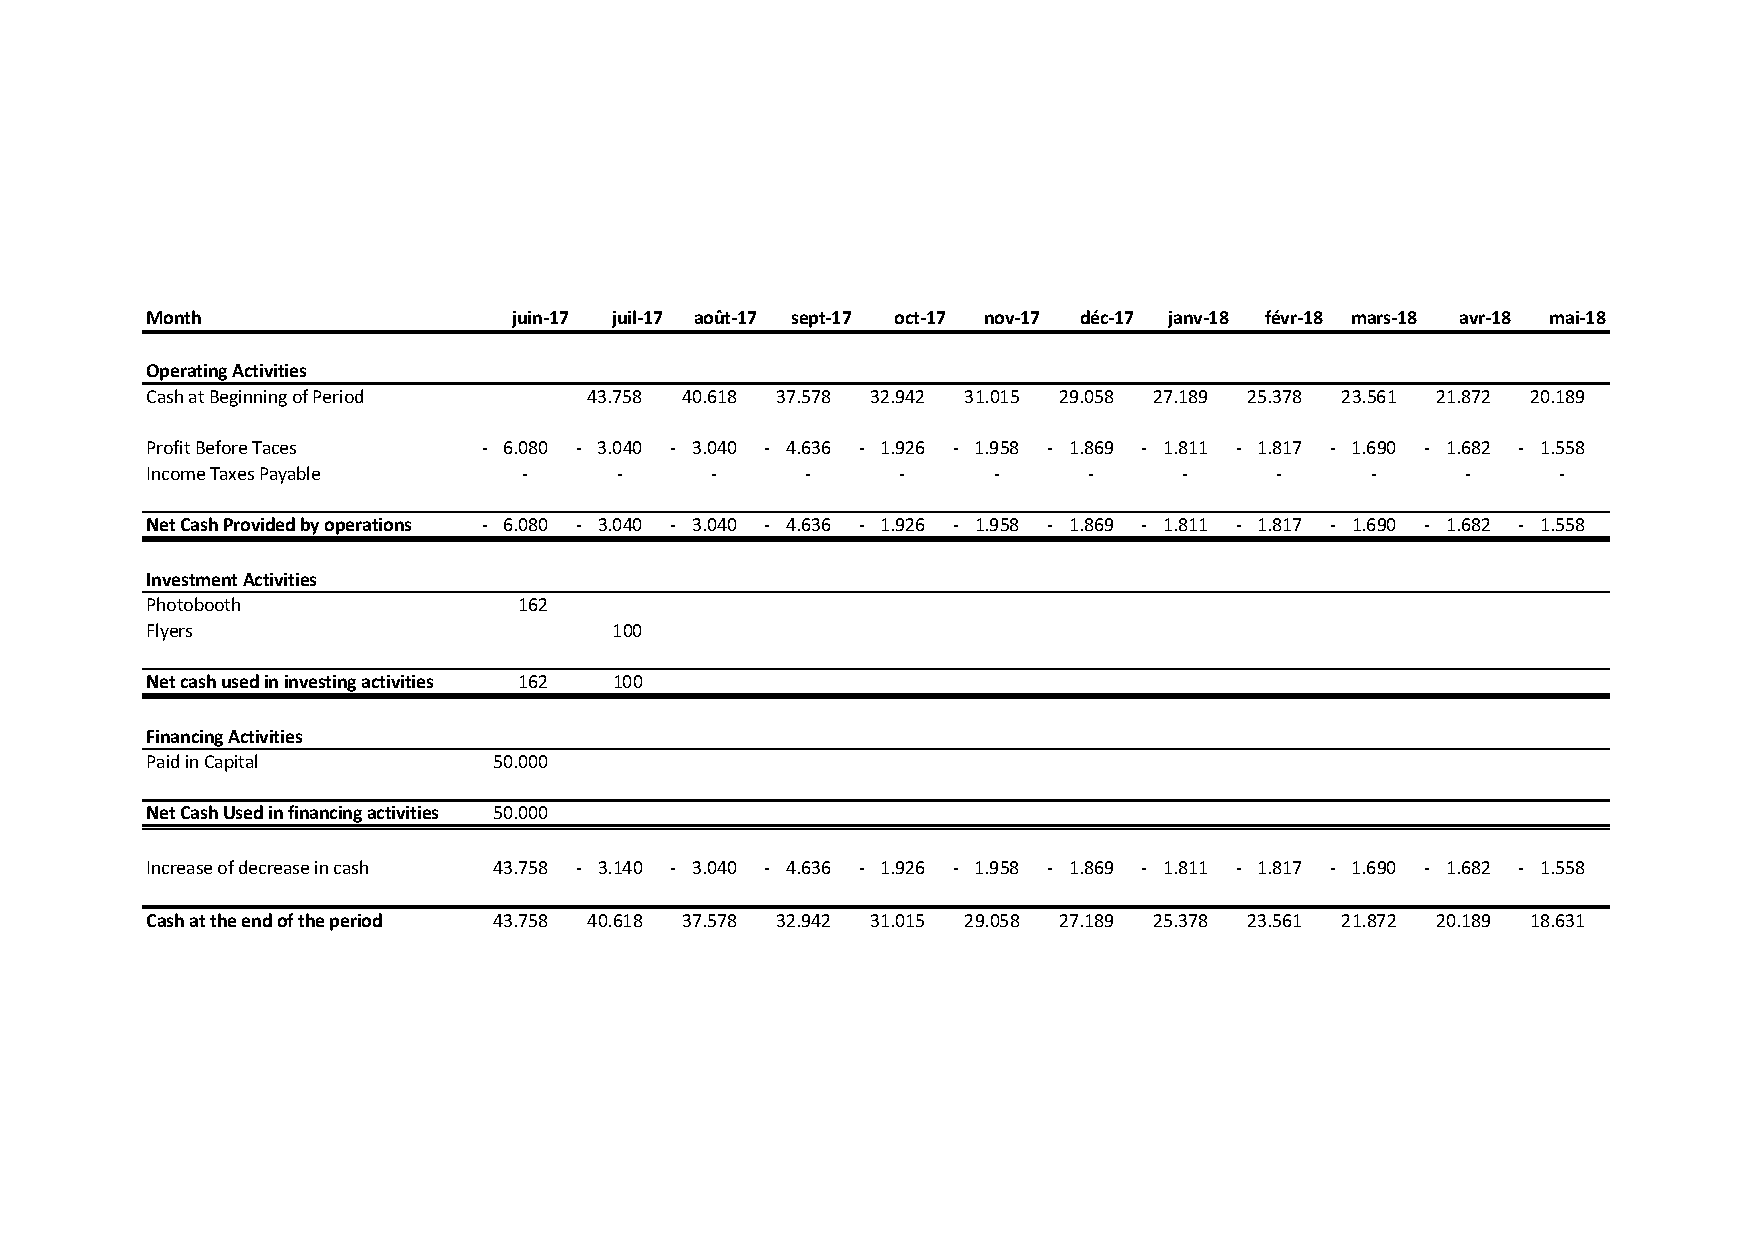
\includepdf[pages={1,2,3},landscape=true]{../sheets/cfs.pdf}

\chapter{Balance Sheet}
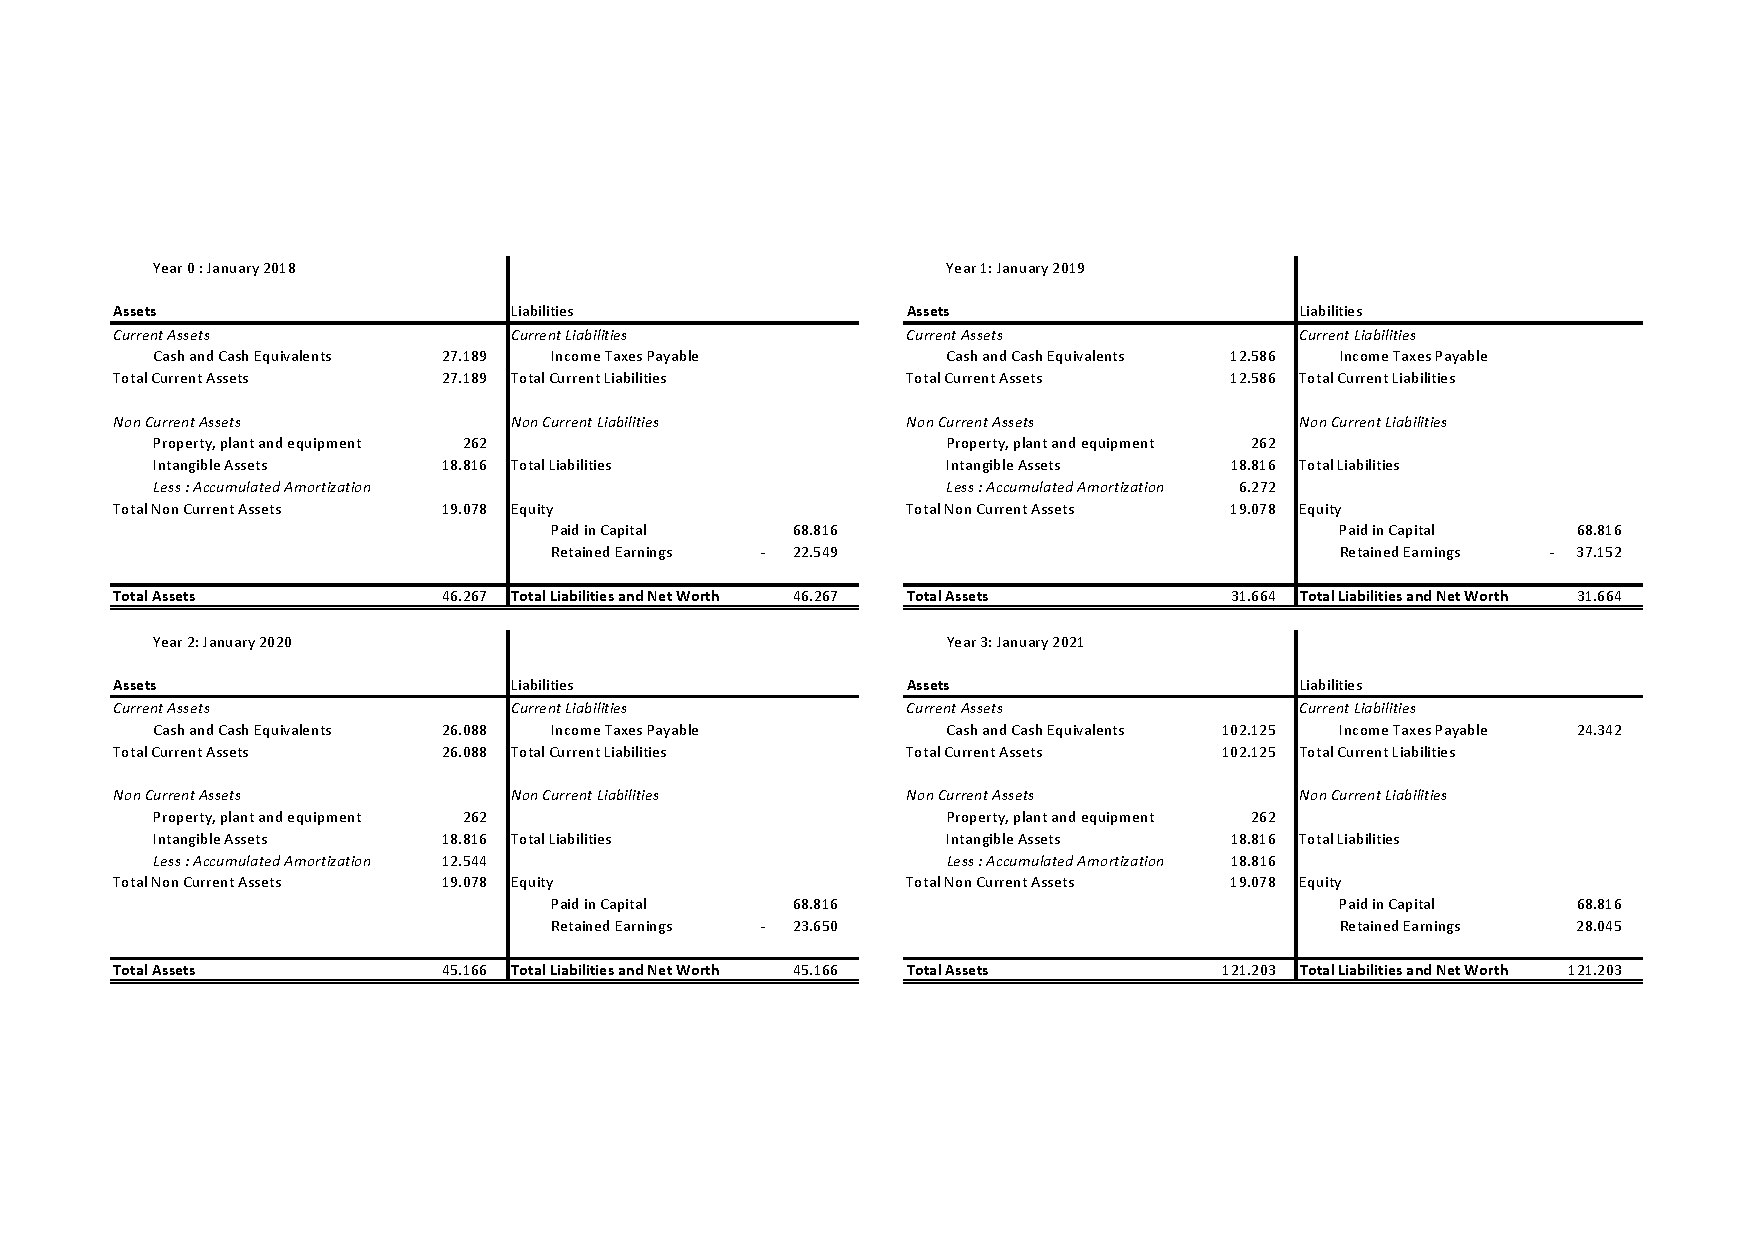
\includepdf[pages={1},landscape=true]{../sheets/bs.pdf}


\end{document}

\end{document}

